\documentclass{article}

\usepackage[left=1.25in,top=1.25in,right=1.25in,bottom=1.25in,head=1.25in]{geometry}
\usepackage{graphicx}

\begin{document}
\begin{figure}[p]
\centering
{\Large\bf $n=100$, $p=10$, Validation tuning} \\
\bigskip
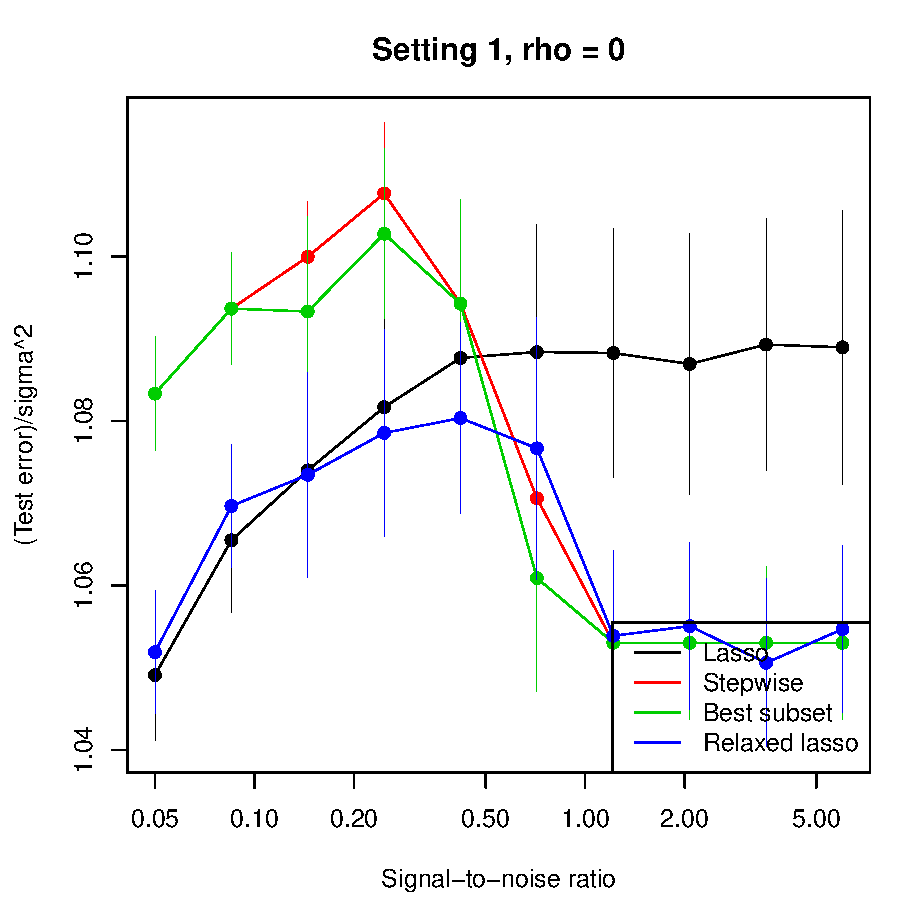
\includegraphics[width=0.32\textwidth]{{fig/val/err.sim.n100.p10.beta1.rho0.00}.pdf}
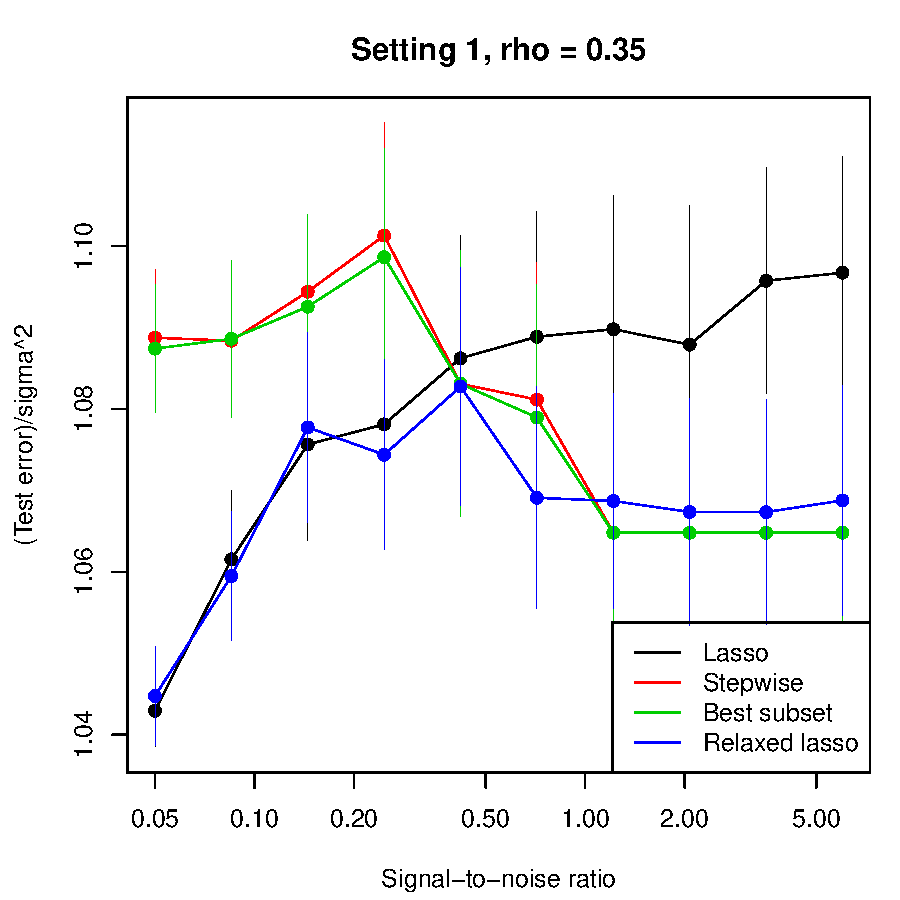
\includegraphics[width=0.32\textwidth]{{fig/val/err.sim.n100.p10.beta1.rho0.35}.pdf}
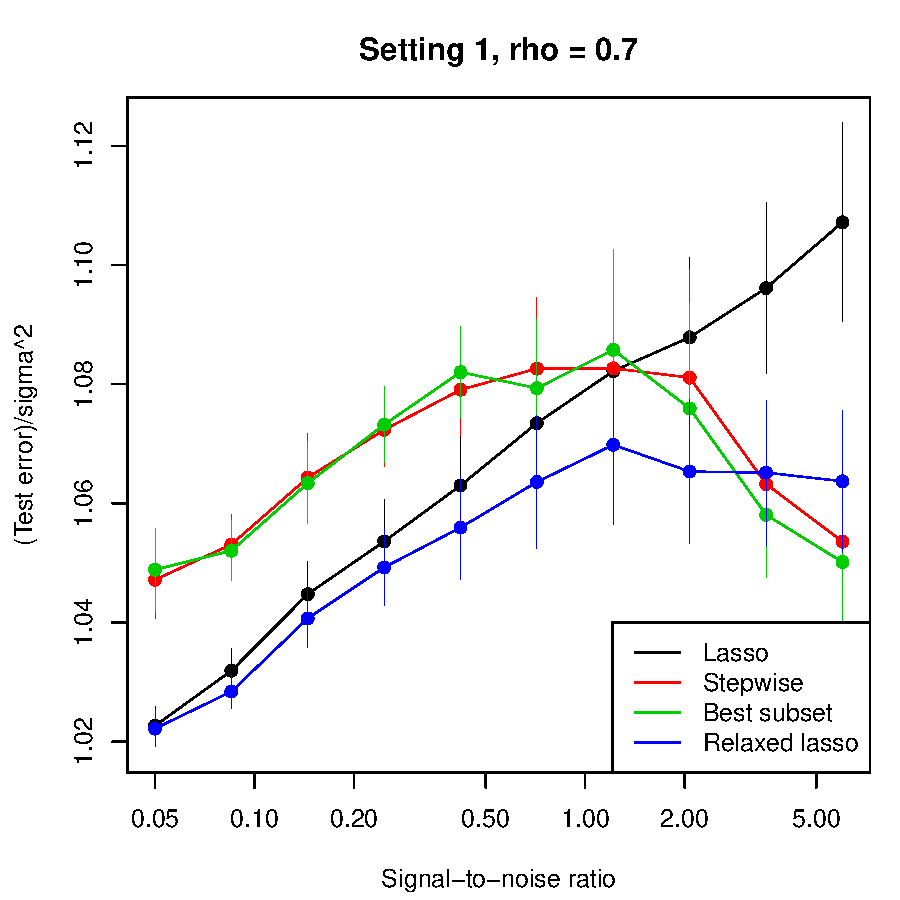
\includegraphics[width=0.32\textwidth]{{fig/val/err.sim.n100.p10.beta1.rho0.70}.pdf}
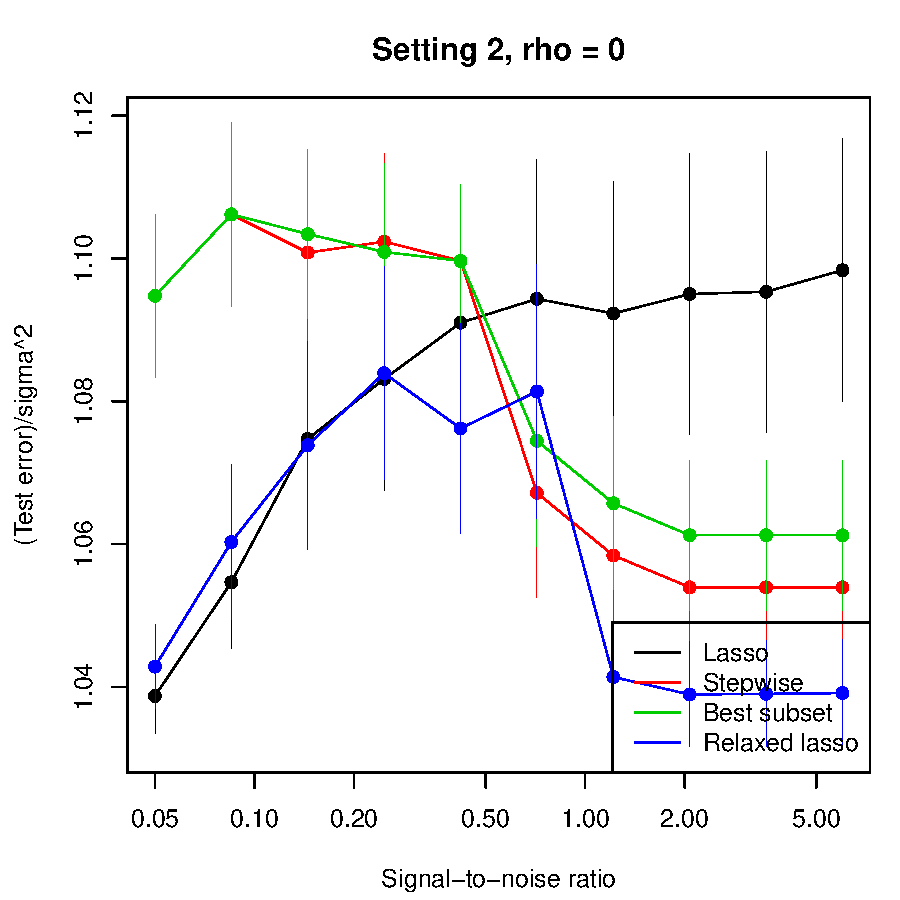
\includegraphics[width=0.32\textwidth]{{fig/val/err.sim.n100.p10.beta2.rho0.00}.pdf}
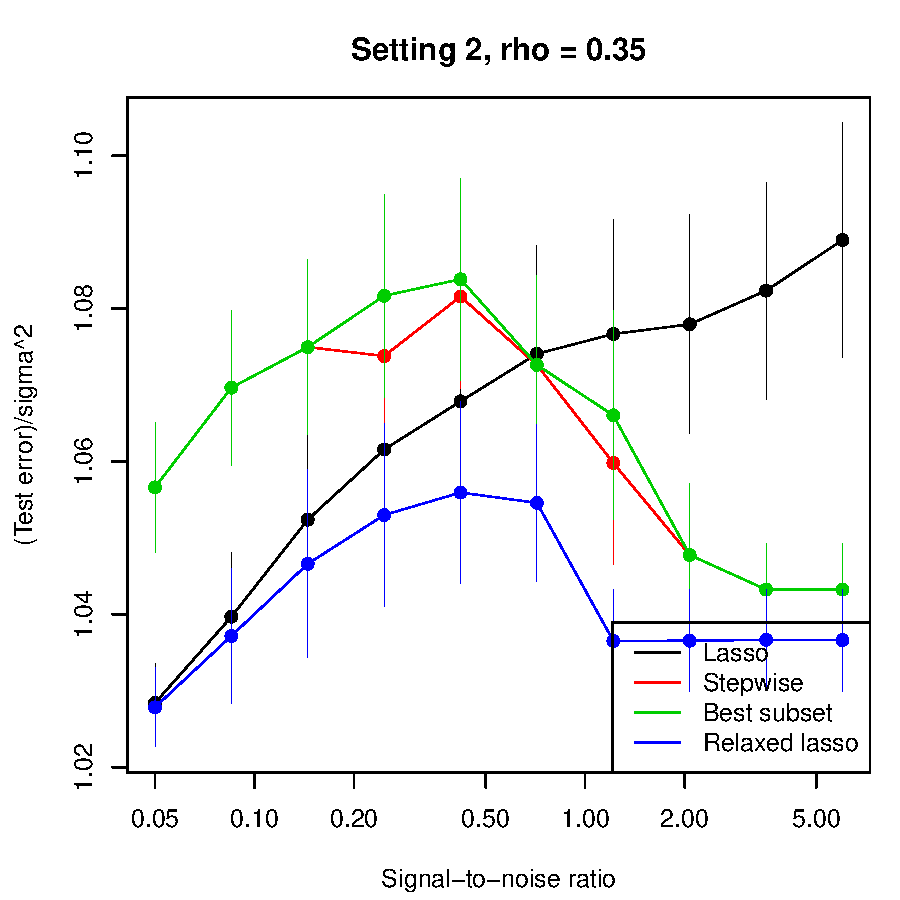
\includegraphics[width=0.32\textwidth]{{fig/val/err.sim.n100.p10.beta2.rho0.35}.pdf}
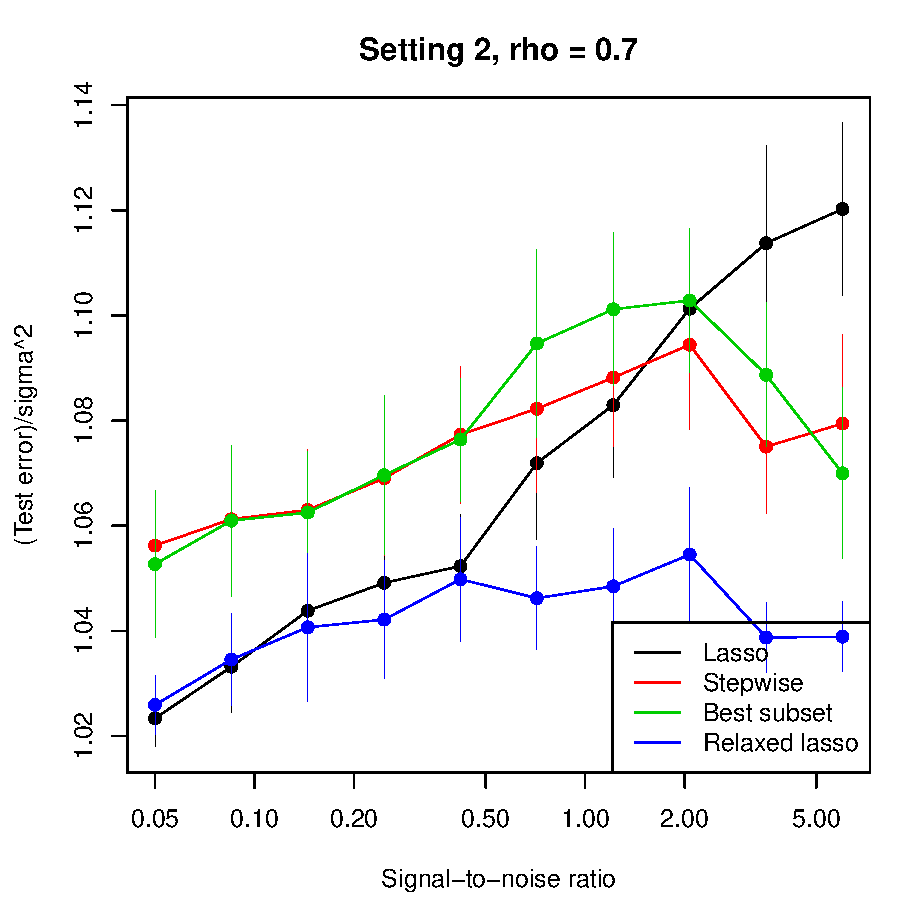
\includegraphics[width=0.32\textwidth]{{fig/val/err.sim.n100.p10.beta2.rho0.70}.pdf}
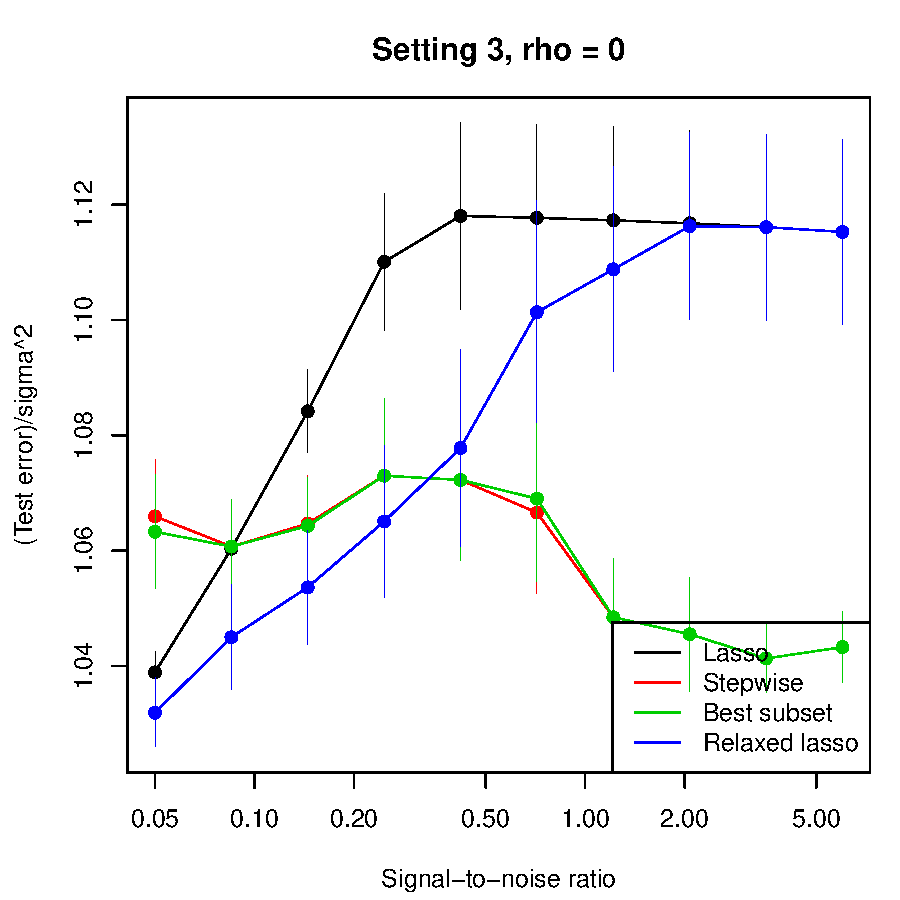
\includegraphics[width=0.32\textwidth]{{fig/val/err.sim.n100.p10.beta3.rho0.00}.pdf}
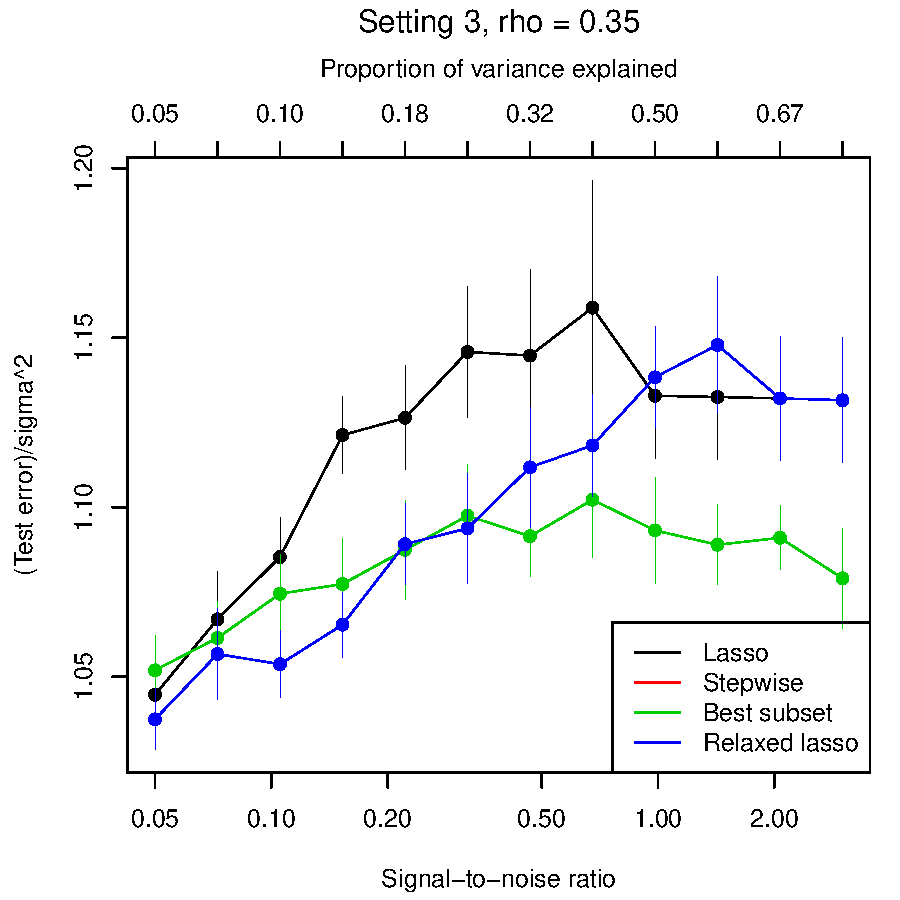
\includegraphics[width=0.32\textwidth]{{fig/val/err.sim.n100.p10.beta3.rho0.35}.pdf}
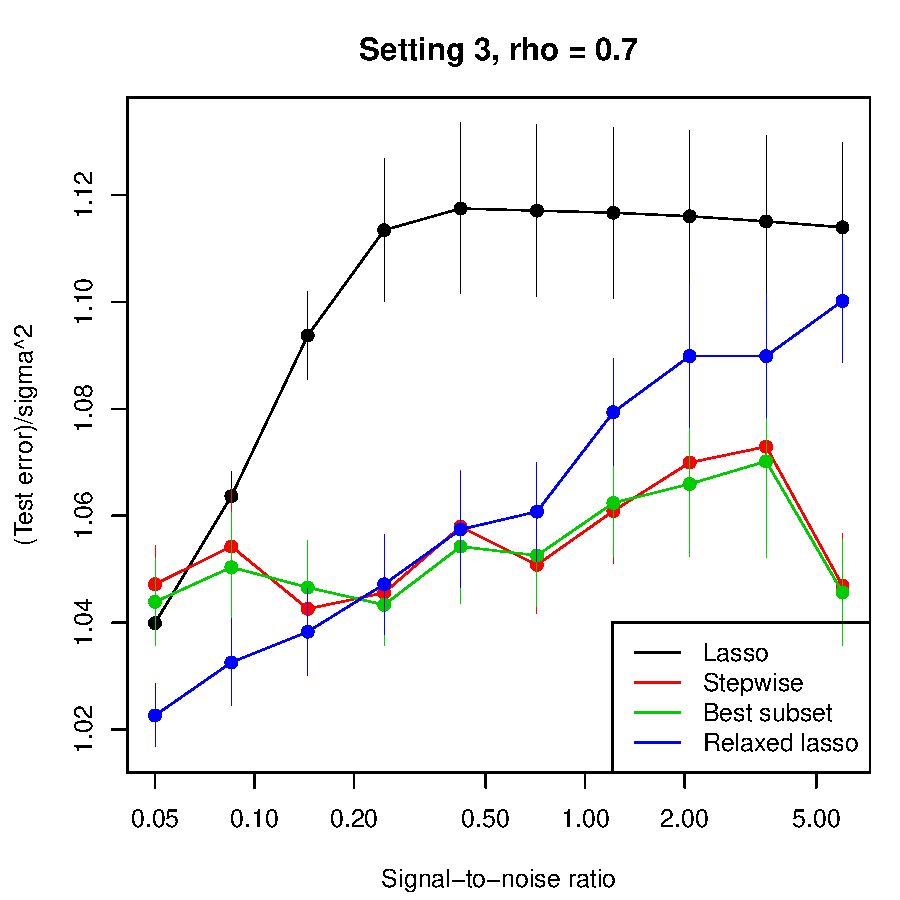
\includegraphics[width=0.32\textwidth]{{fig/val/err.sim.n100.p10.beta3.rho0.70}.pdf}
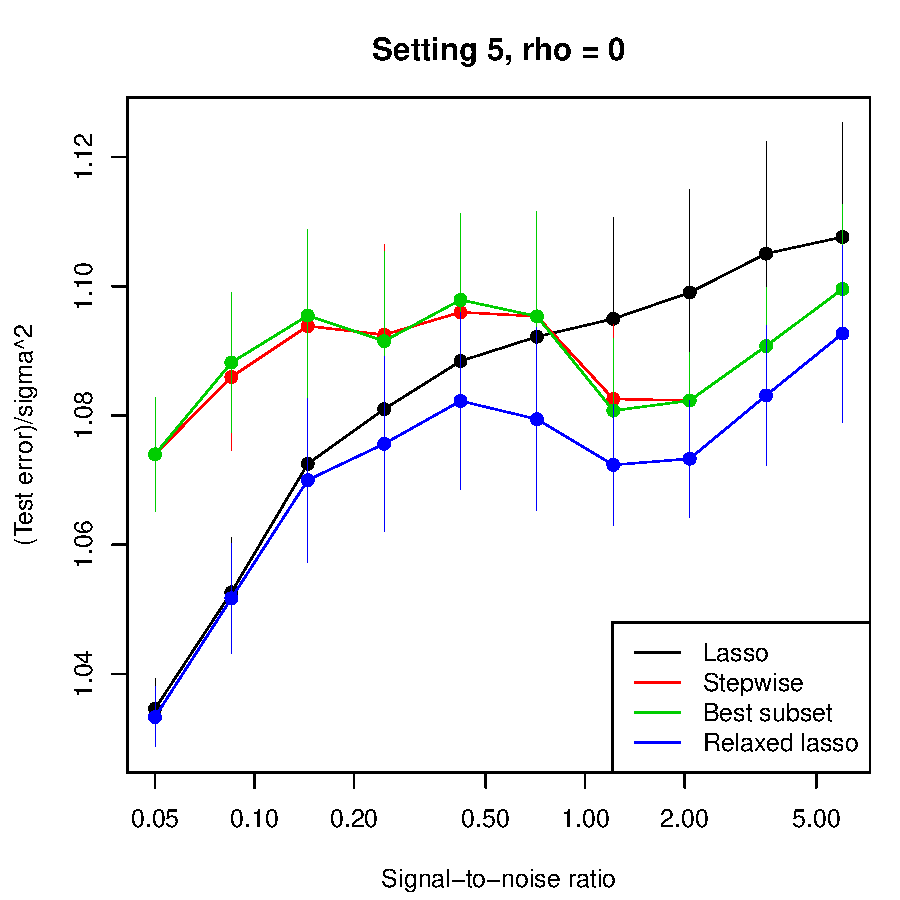
\includegraphics[width=0.32\textwidth]{{fig/val/err.sim.n100.p10.beta5.rho0.00}.pdf}
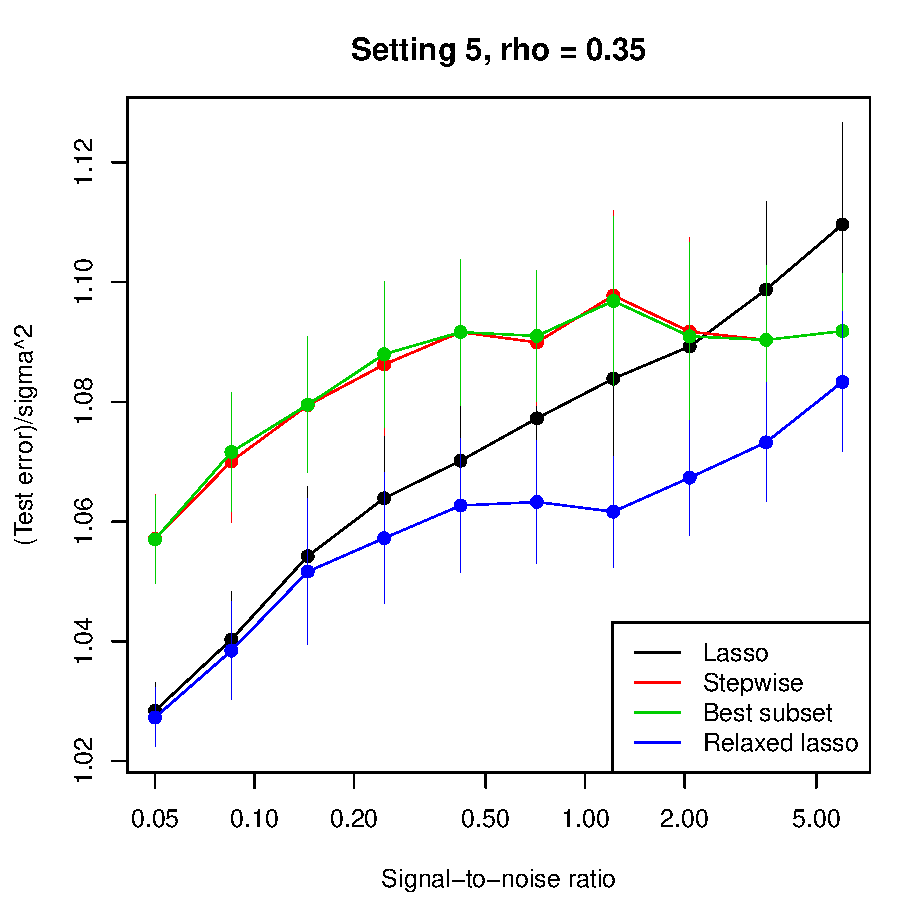
\includegraphics[width=0.32\textwidth]{{fig/val/err.sim.n100.p10.beta5.rho0.35}.pdf}
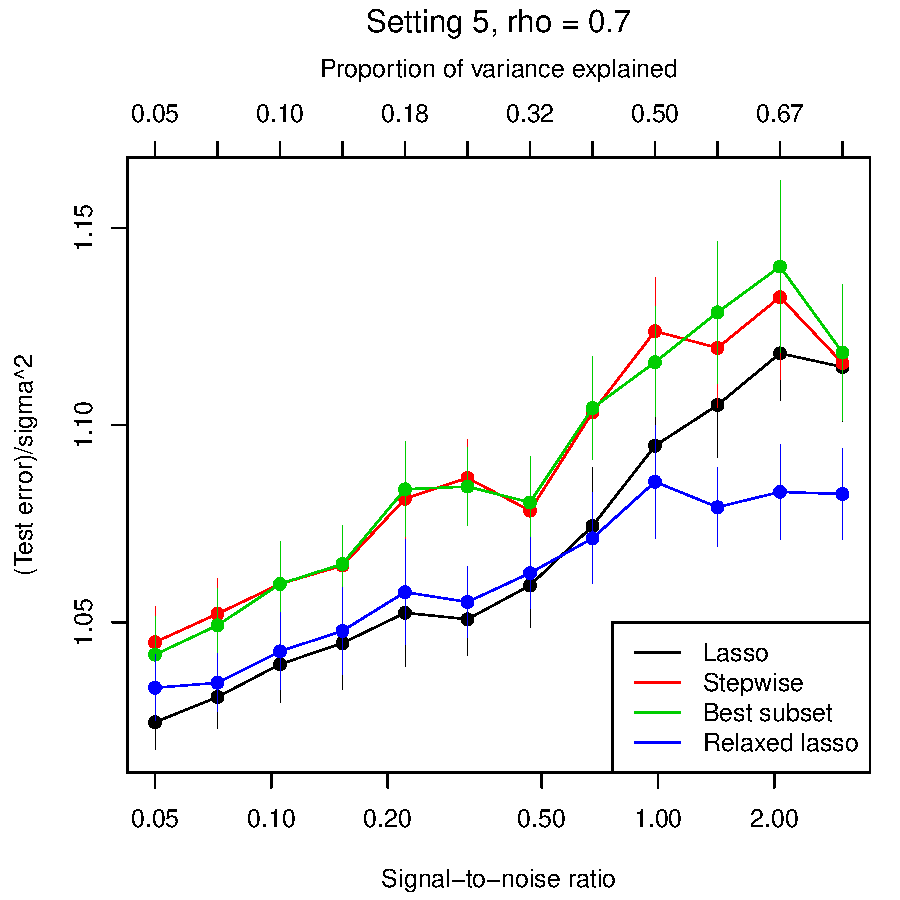
\includegraphics[width=0.32\textwidth]{{fig/val/err.sim.n100.p10.beta5.rho0.70}.pdf}

\end{figure}

\begin{figure}[p]
\centering
{\Large\bf $n=100$, $p=10$, Validation tuning} \\
\bigskip
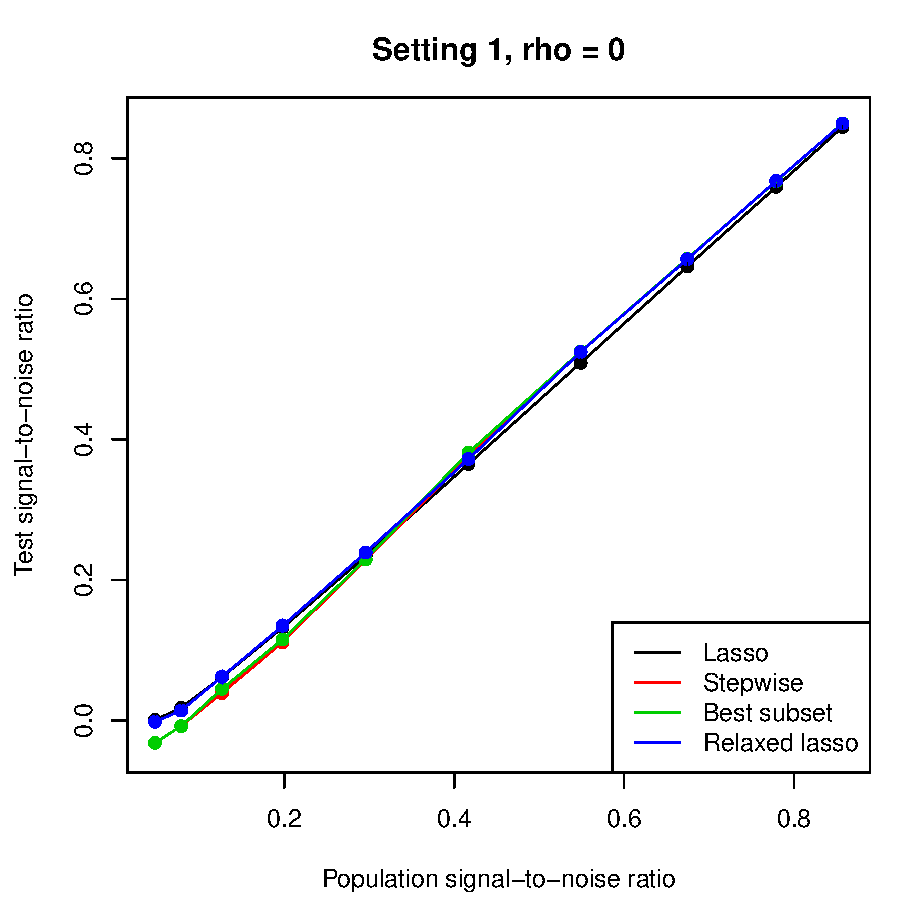
\includegraphics[width=0.32\textwidth]{{fig/val/pro.sim.n100.p10.beta1.rho0.00}.pdf}
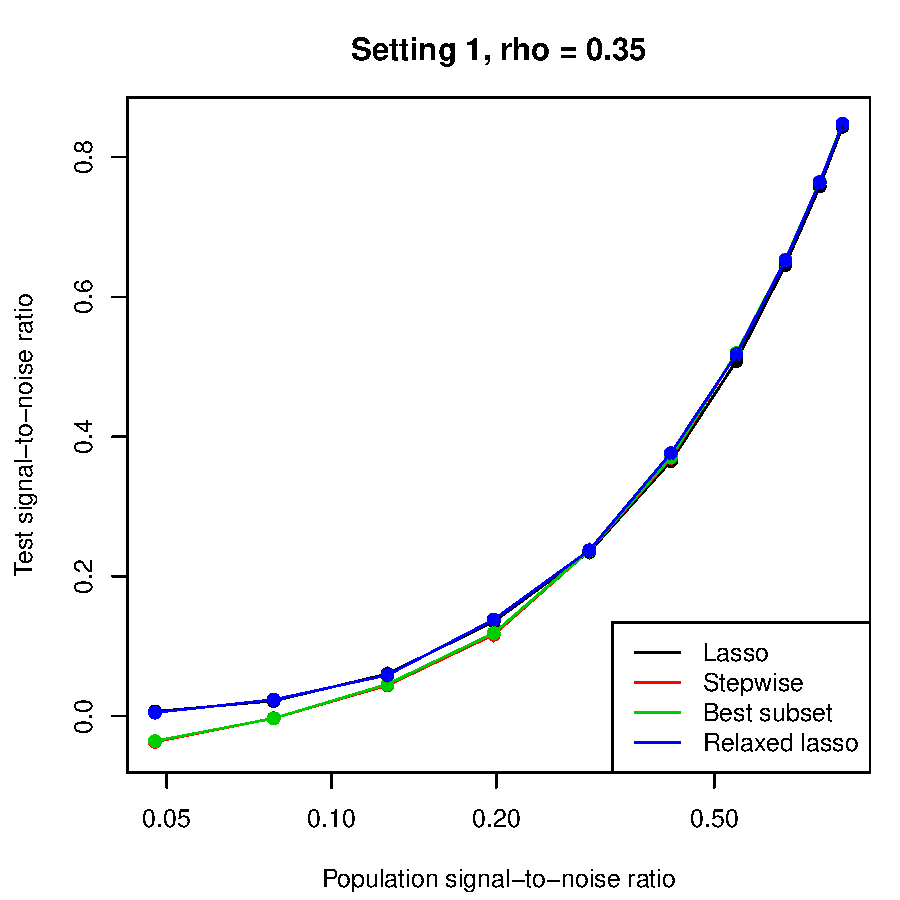
\includegraphics[width=0.32\textwidth]{{fig/val/pro.sim.n100.p10.beta1.rho0.35}.pdf}
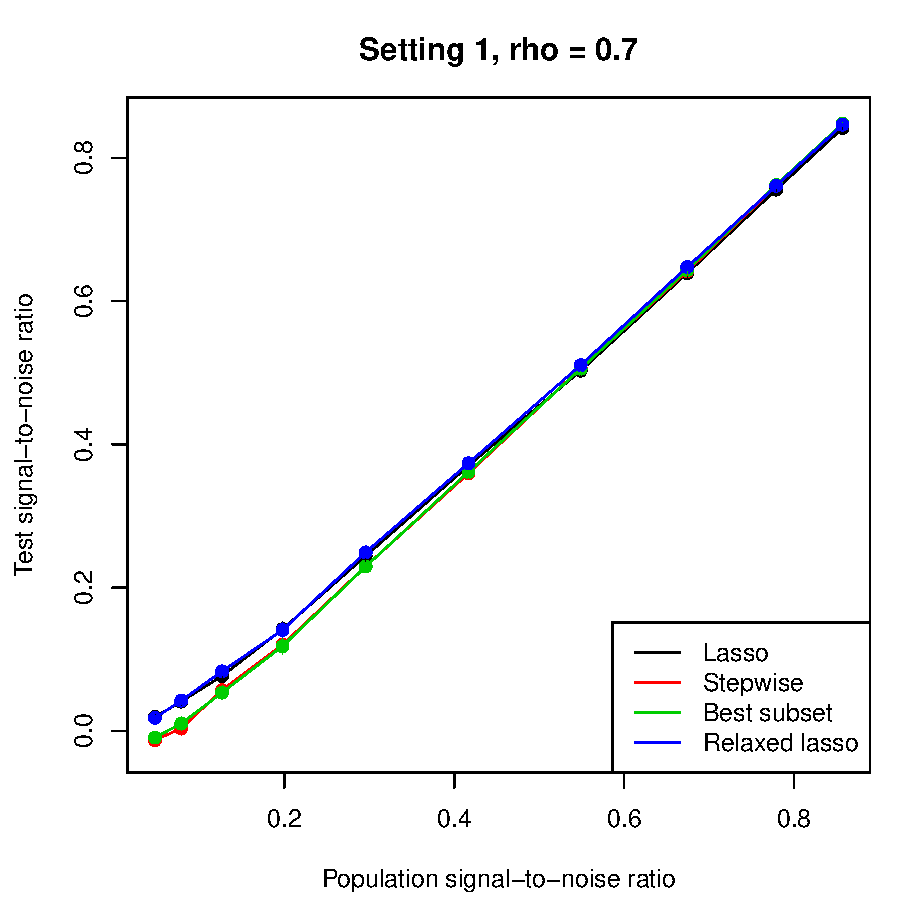
\includegraphics[width=0.32\textwidth]{{fig/val/pro.sim.n100.p10.beta1.rho0.70}.pdf}
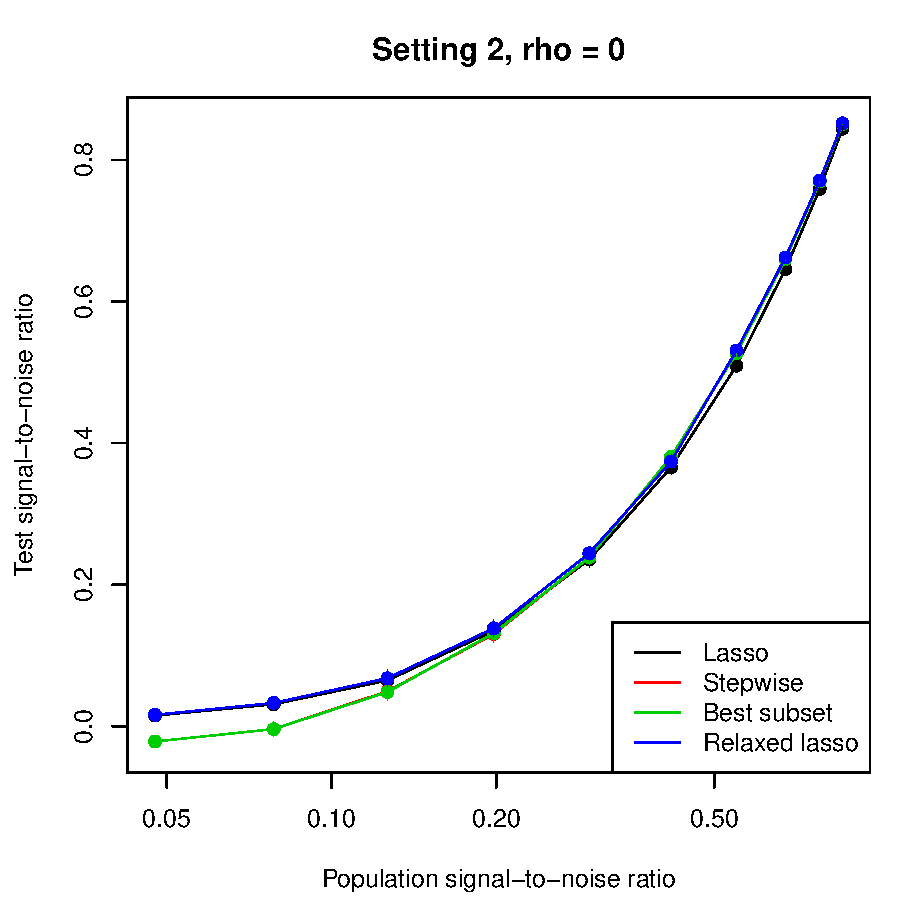
\includegraphics[width=0.32\textwidth]{{fig/val/pro.sim.n100.p10.beta2.rho0.00}.pdf}
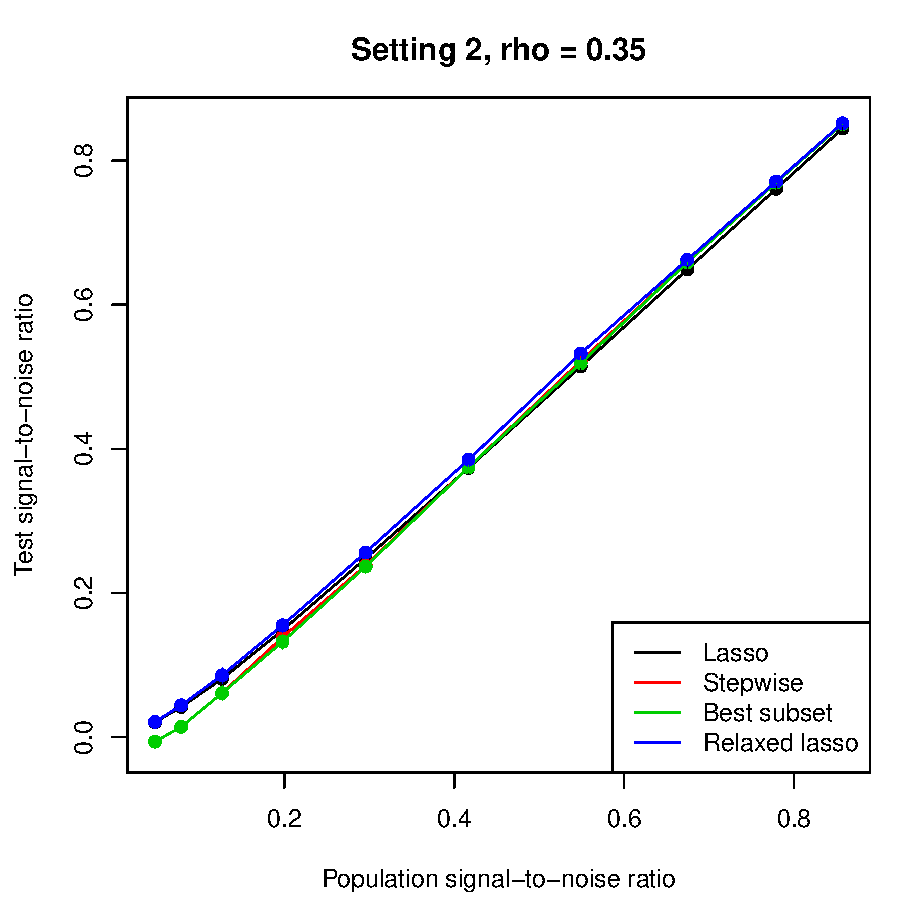
\includegraphics[width=0.32\textwidth]{{fig/val/pro.sim.n100.p10.beta2.rho0.35}.pdf}
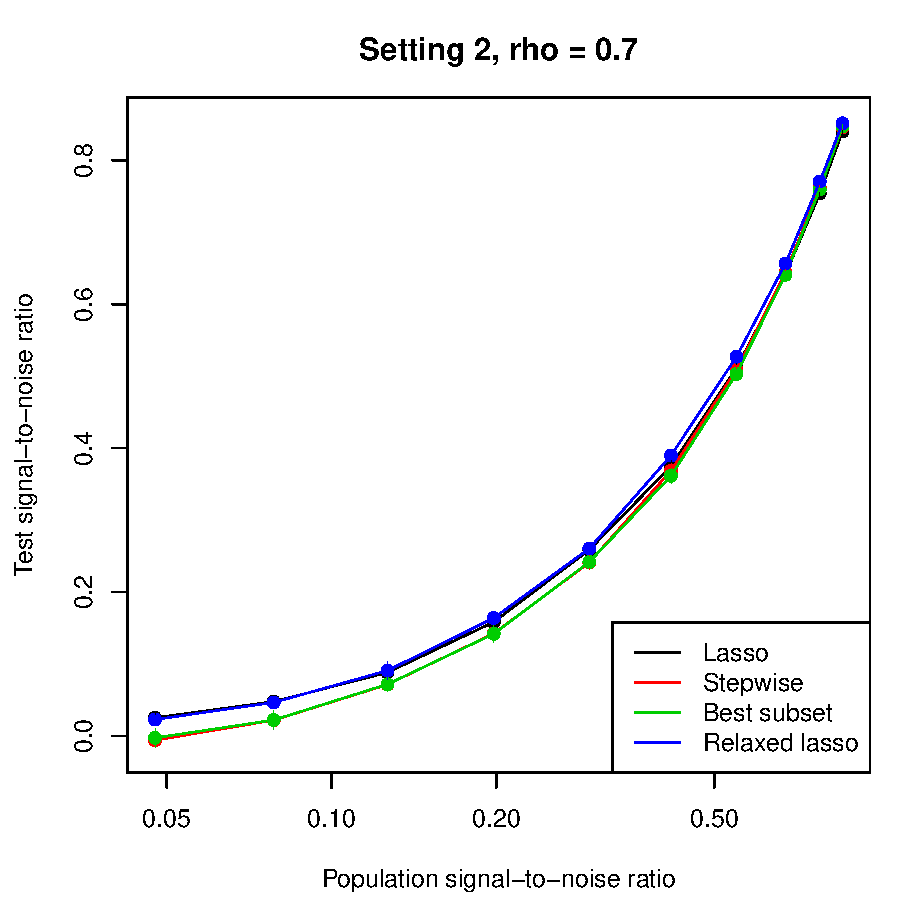
\includegraphics[width=0.32\textwidth]{{fig/val/pro.sim.n100.p10.beta2.rho0.70}.pdf}
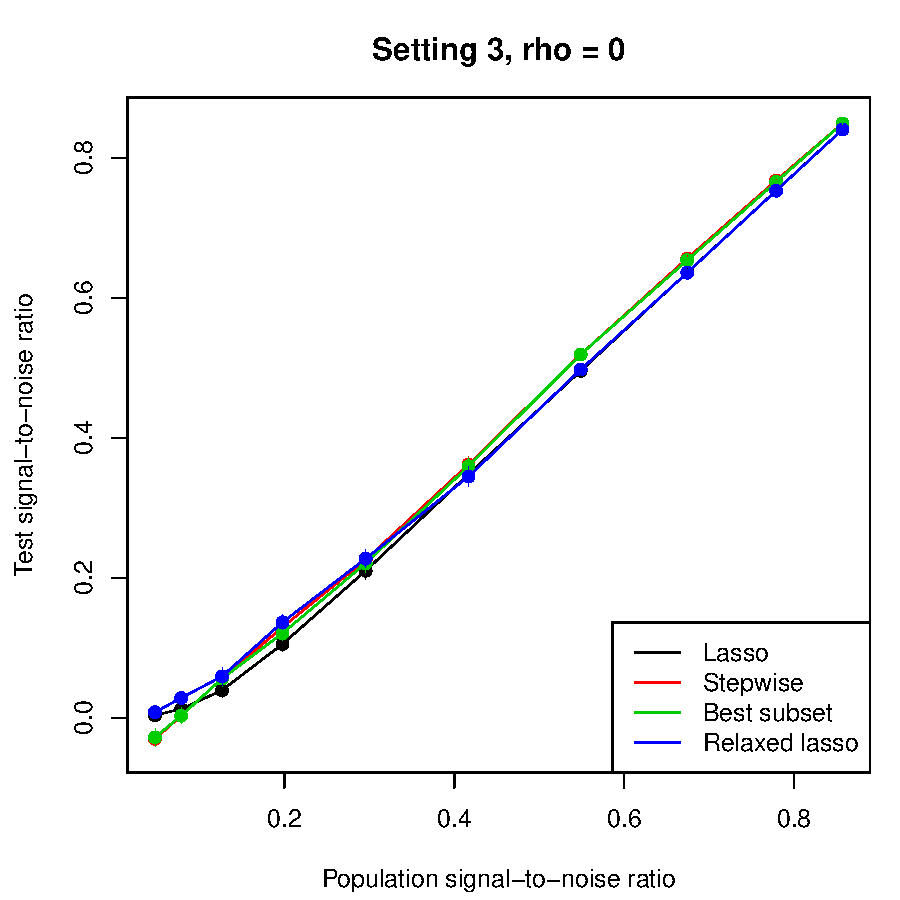
\includegraphics[width=0.32\textwidth]{{fig/val/pro.sim.n100.p10.beta3.rho0.00}.pdf}
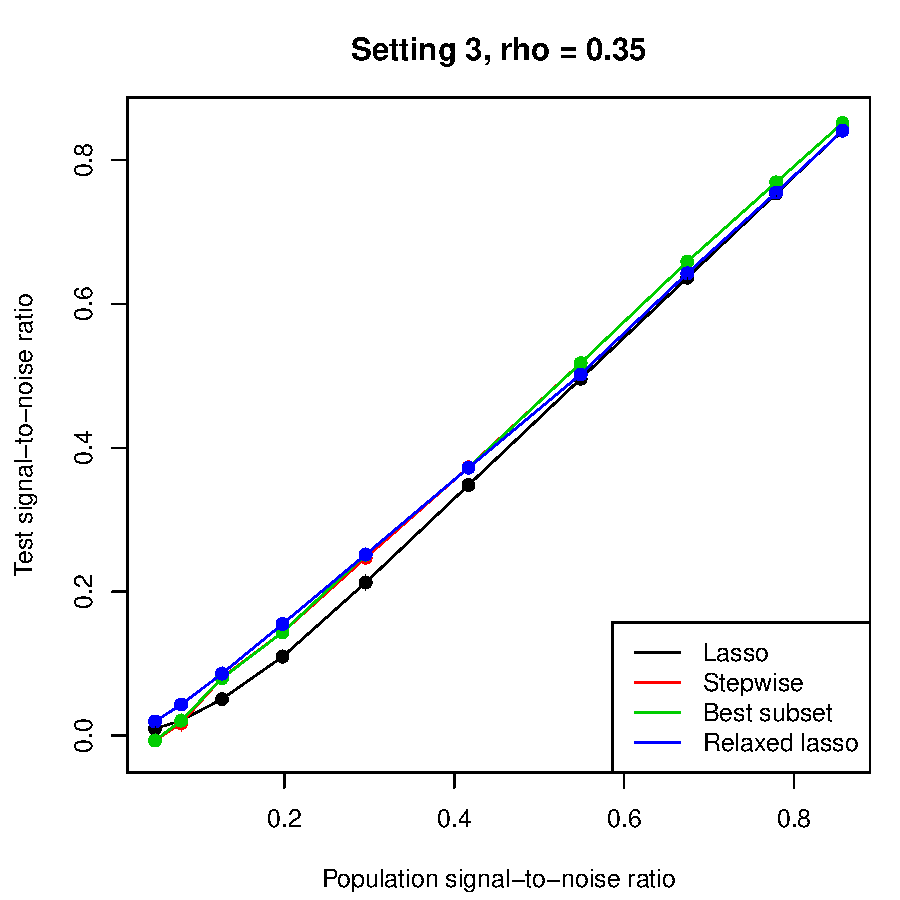
\includegraphics[width=0.32\textwidth]{{fig/val/pro.sim.n100.p10.beta3.rho0.35}.pdf}
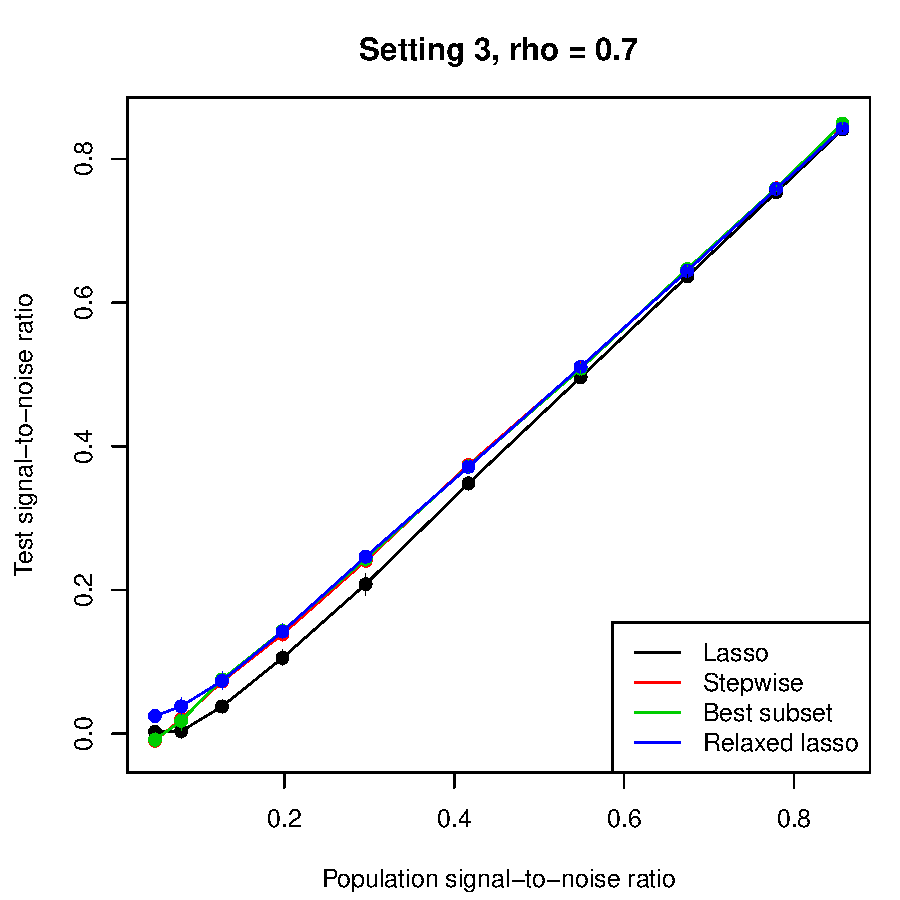
\includegraphics[width=0.32\textwidth]{{fig/val/pro.sim.n100.p10.beta3.rho0.70}.pdf}
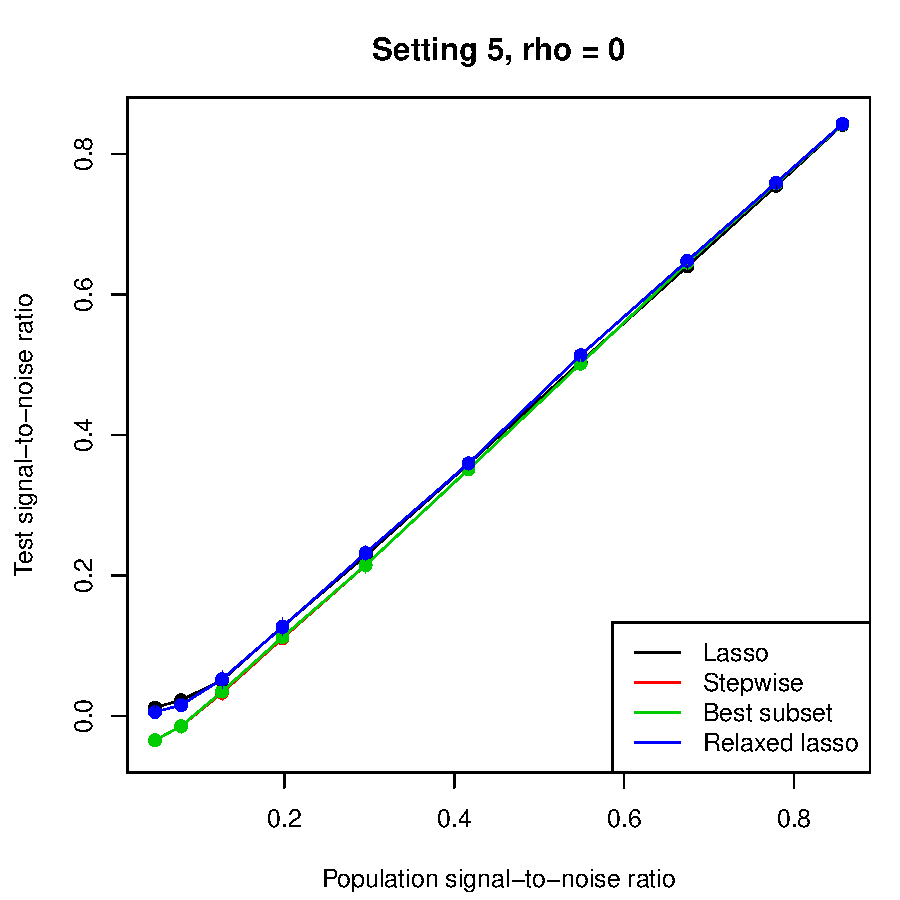
\includegraphics[width=0.32\textwidth]{{fig/val/pro.sim.n100.p10.beta5.rho0.00}.pdf}
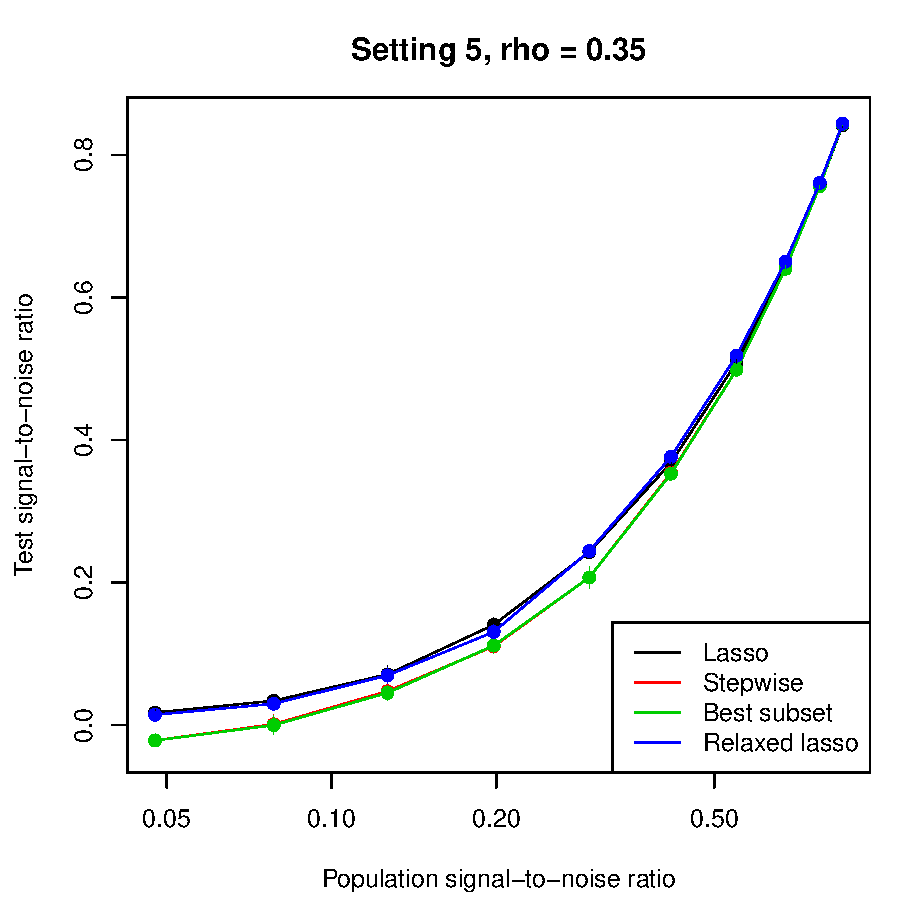
\includegraphics[width=0.32\textwidth]{{fig/val/pro.sim.n100.p10.beta5.rho0.35}.pdf}
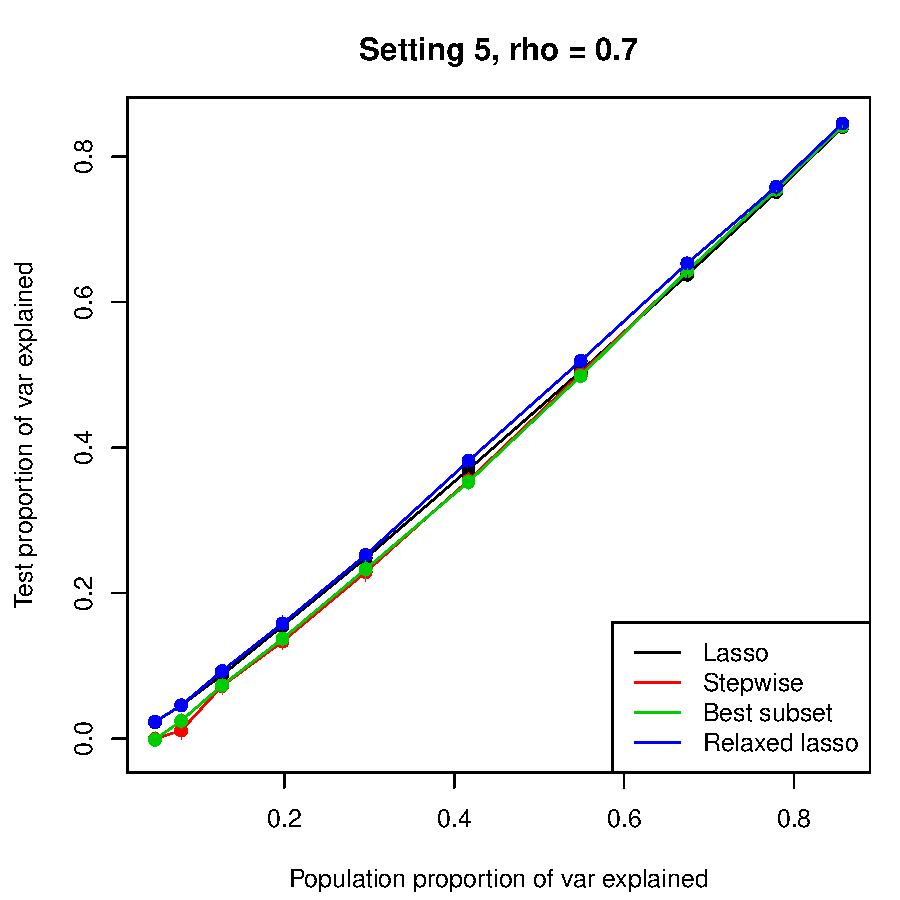
\includegraphics[width=0.32\textwidth]{{fig/val/pro.sim.n100.p10.beta5.rho0.70}.pdf}

\end{figure}

\begin{figure}[p]
\centering
{\Large\bf $n=100$, $p=10$, Validation tuning} \\
\bigskip
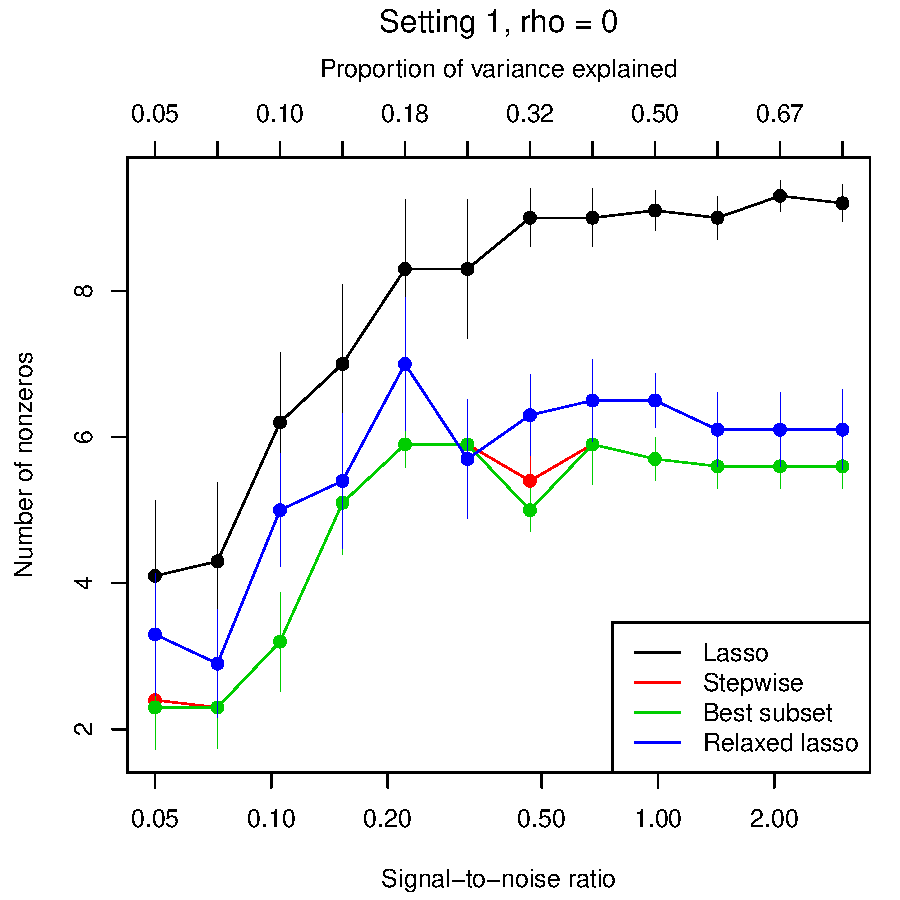
\includegraphics[width=0.32\textwidth]{{fig/val/nzs.sim.n100.p10.beta1.rho0.00}.pdf}
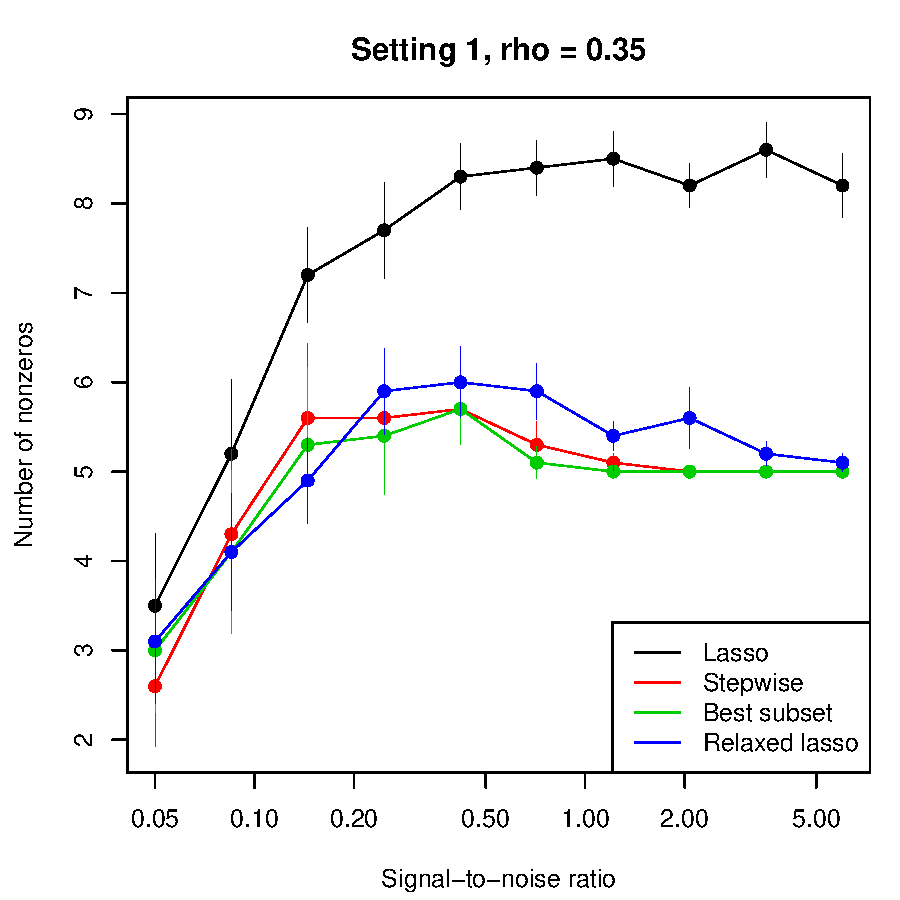
\includegraphics[width=0.32\textwidth]{{fig/val/nzs.sim.n100.p10.beta1.rho0.35}.pdf}
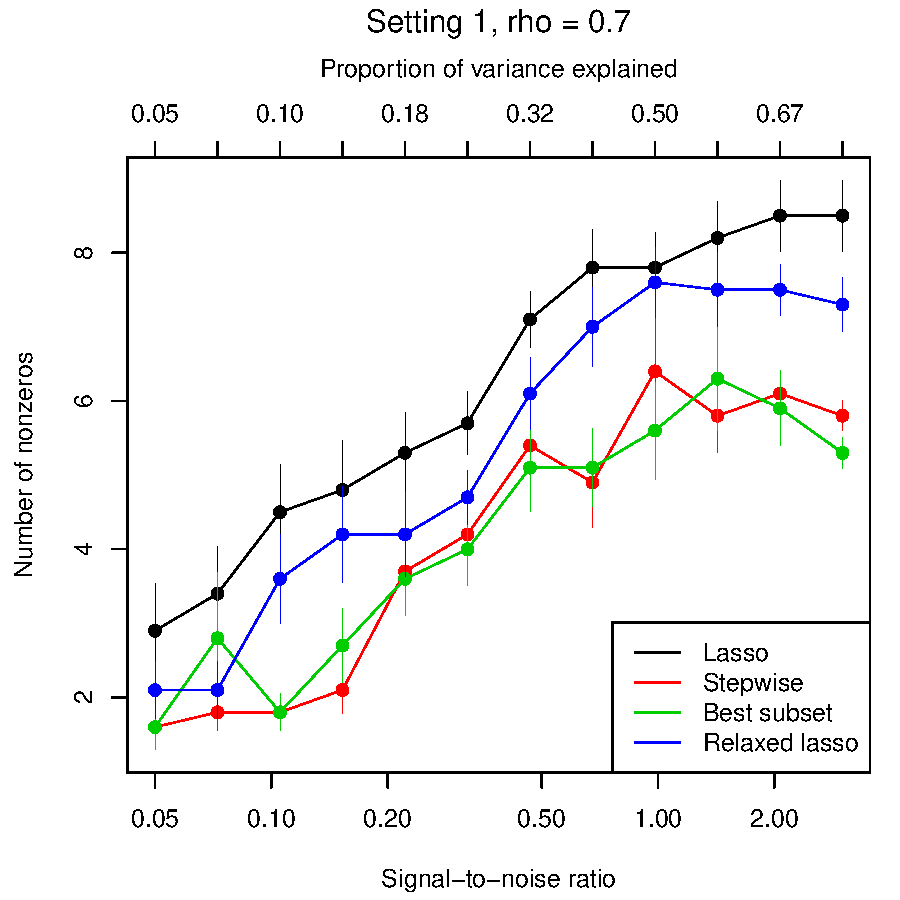
\includegraphics[width=0.32\textwidth]{{fig/val/nzs.sim.n100.p10.beta1.rho0.70}.pdf}
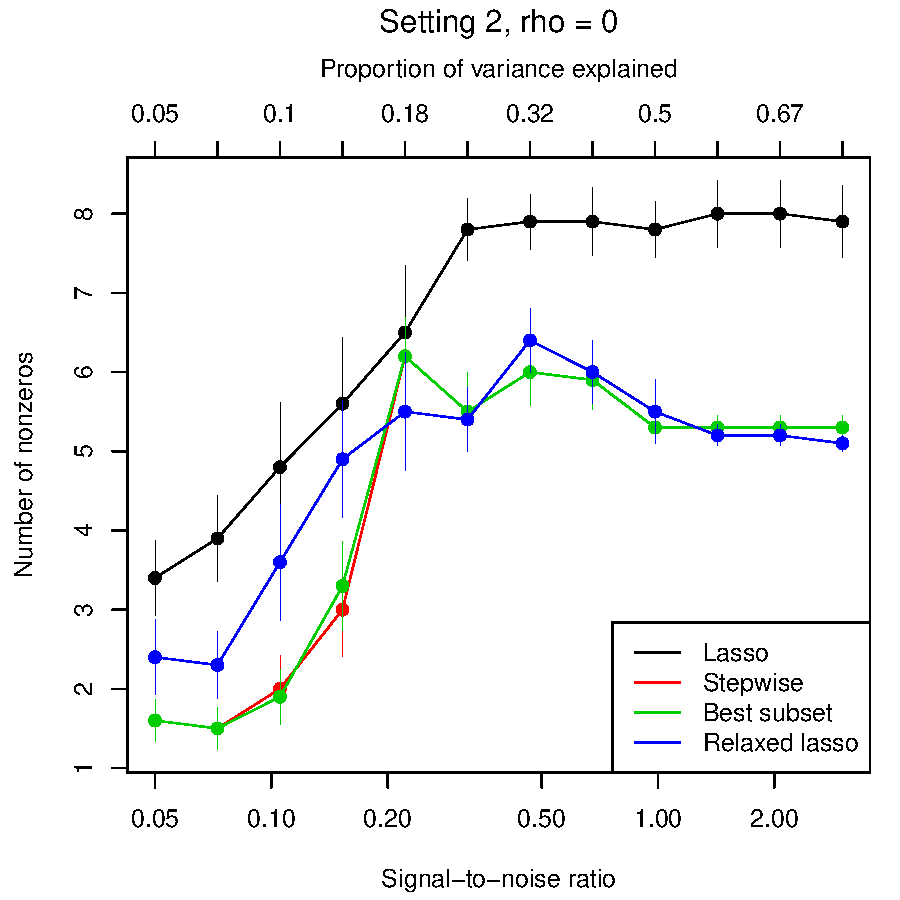
\includegraphics[width=0.32\textwidth]{{fig/val/nzs.sim.n100.p10.beta2.rho0.00}.pdf}
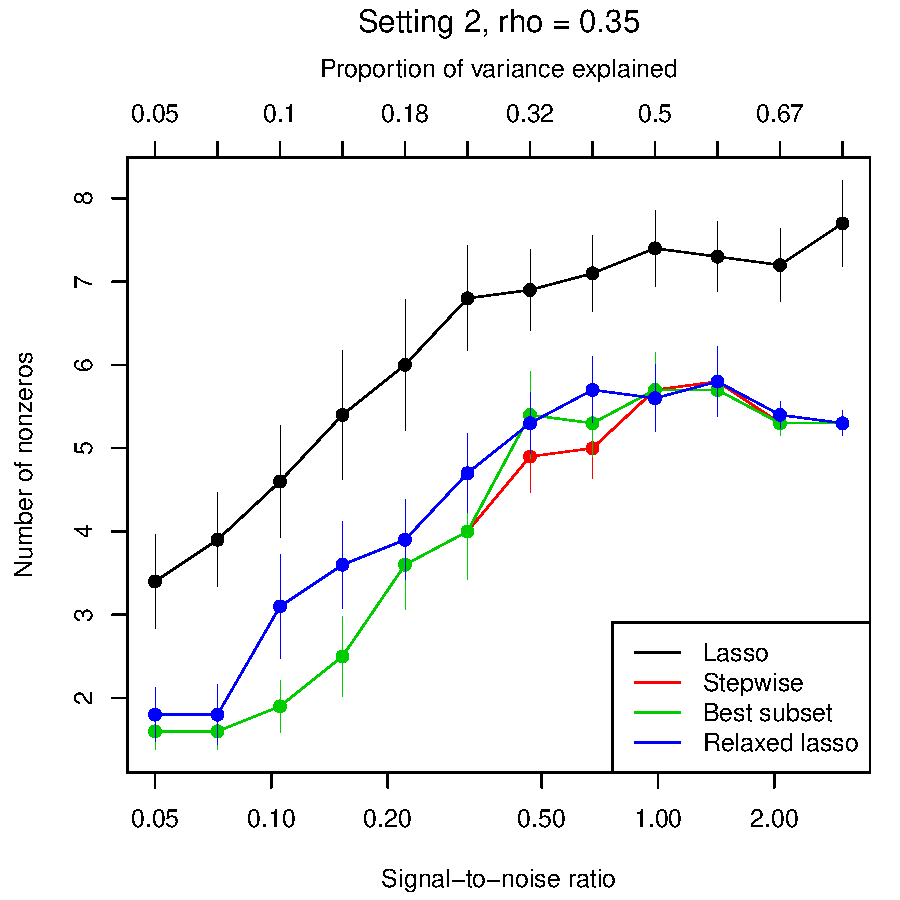
\includegraphics[width=0.32\textwidth]{{fig/val/nzs.sim.n100.p10.beta2.rho0.35}.pdf}
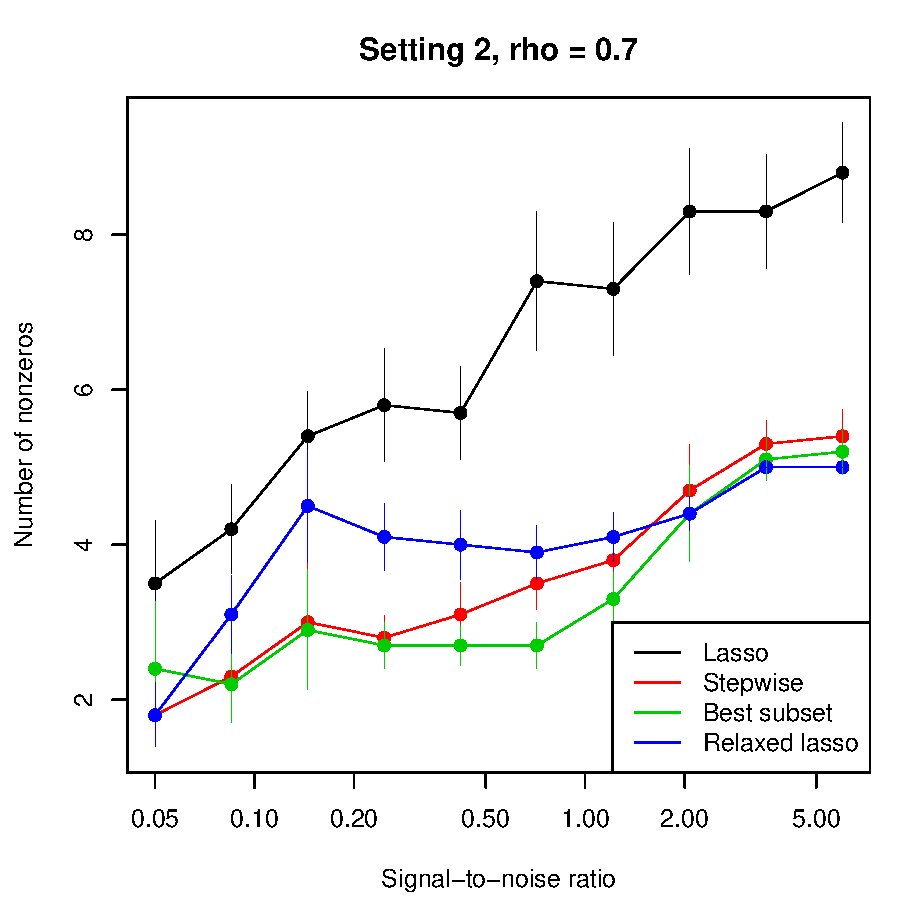
\includegraphics[width=0.32\textwidth]{{fig/val/nzs.sim.n100.p10.beta2.rho0.70}.pdf}
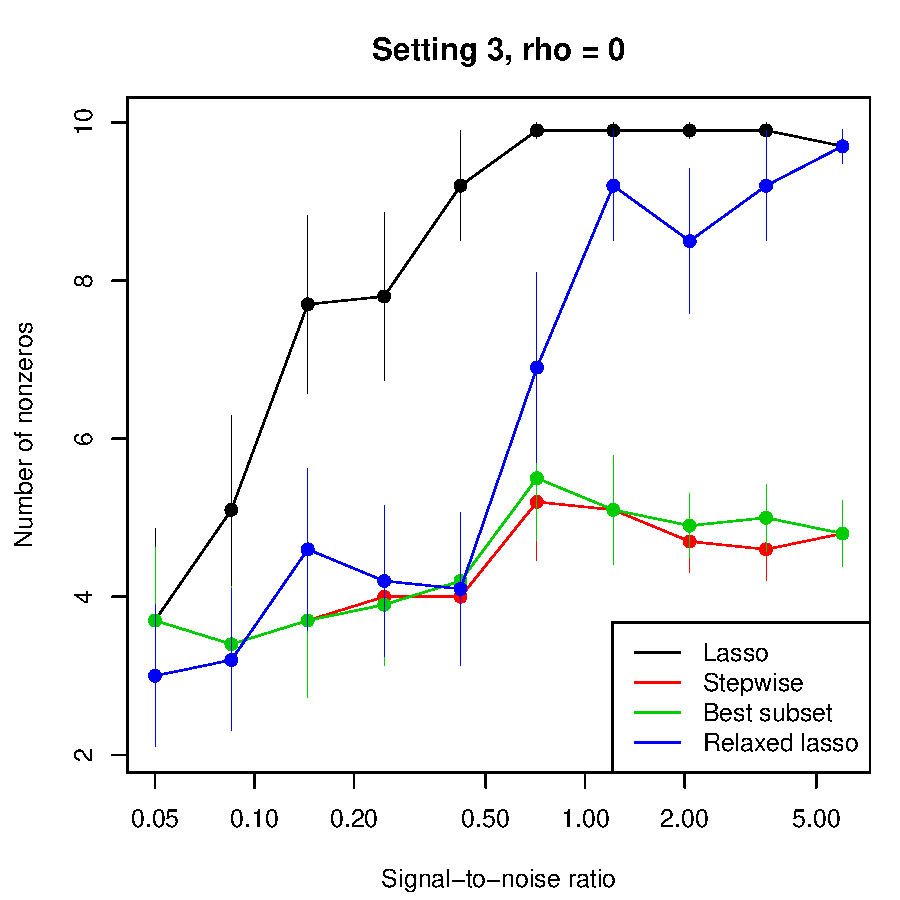
\includegraphics[width=0.32\textwidth]{{fig/val/nzs.sim.n100.p10.beta3.rho0.00}.pdf}
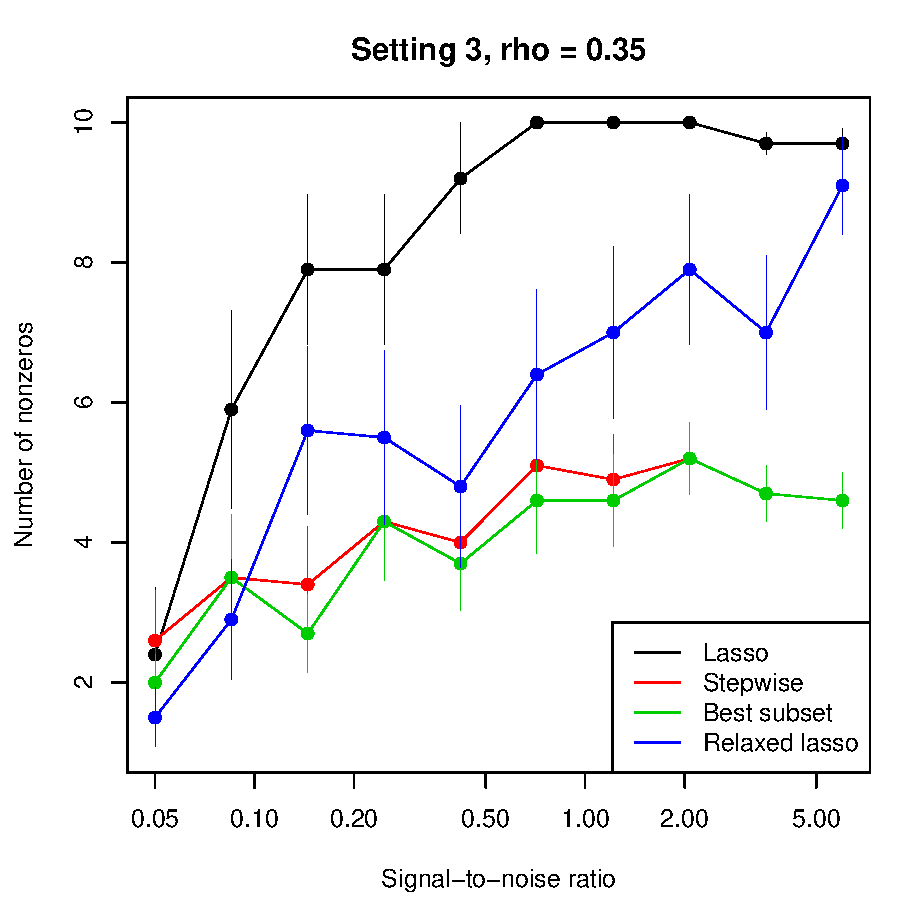
\includegraphics[width=0.32\textwidth]{{fig/val/nzs.sim.n100.p10.beta3.rho0.35}.pdf}
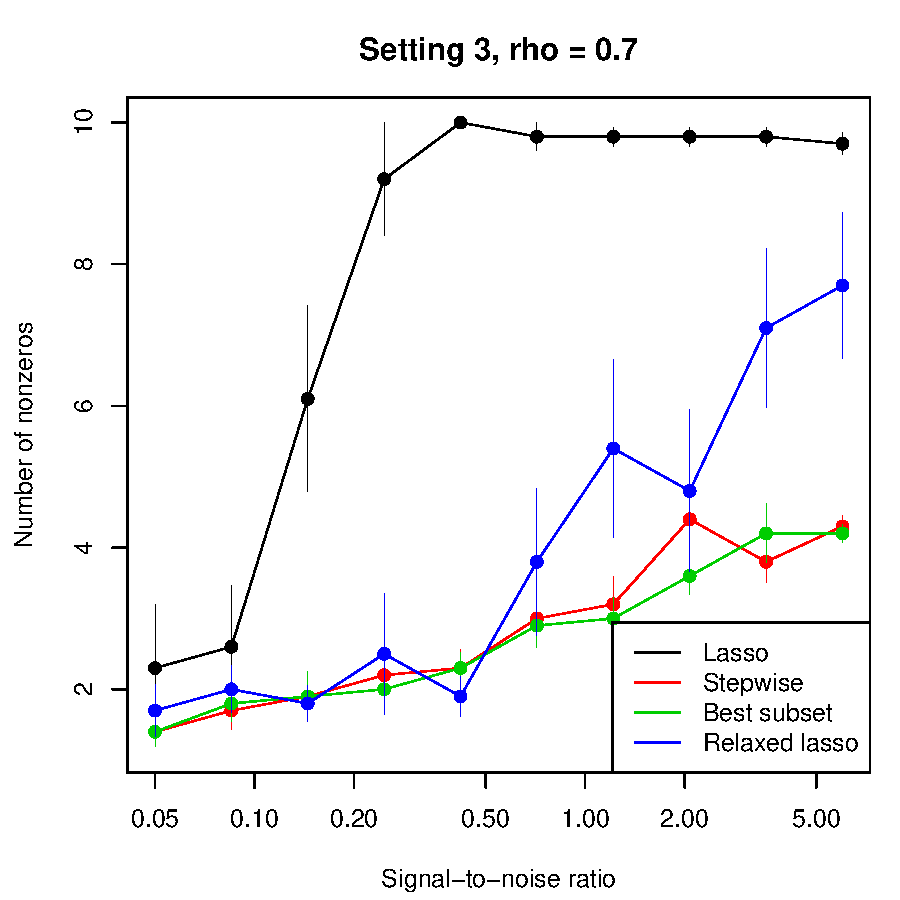
\includegraphics[width=0.32\textwidth]{{fig/val/nzs.sim.n100.p10.beta3.rho0.70}.pdf}
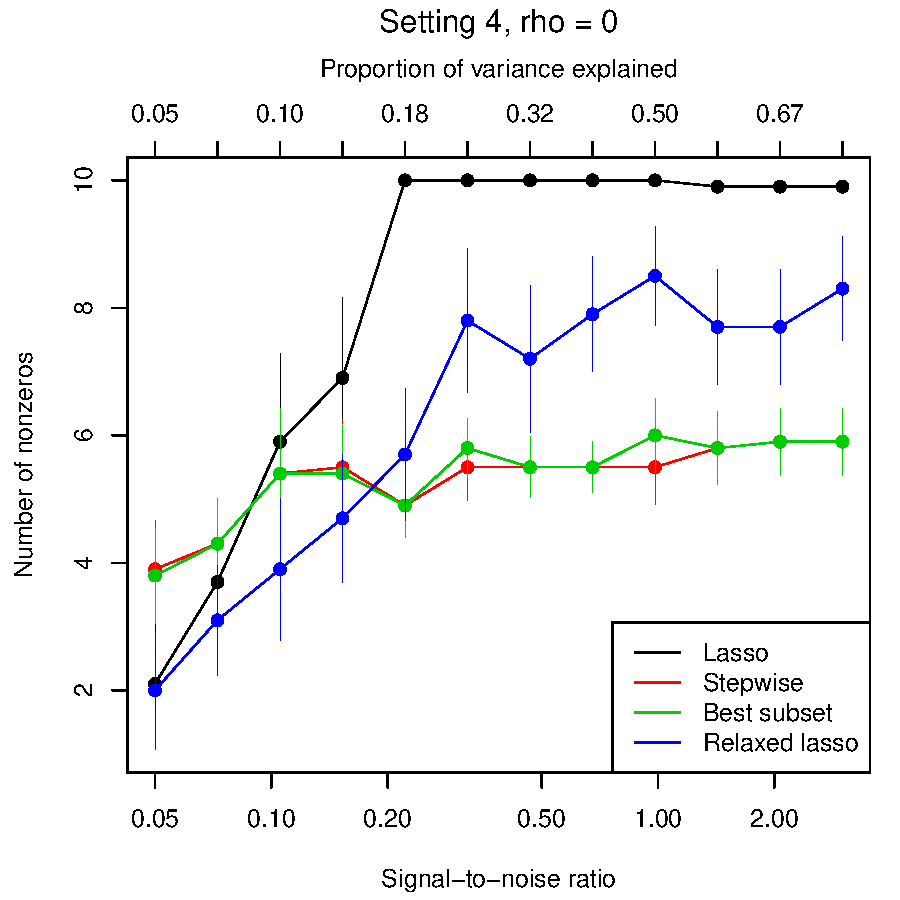
\includegraphics[width=0.32\textwidth]{{fig/val/nzs.sim.n100.p10.beta4.rho0.00}.pdf}
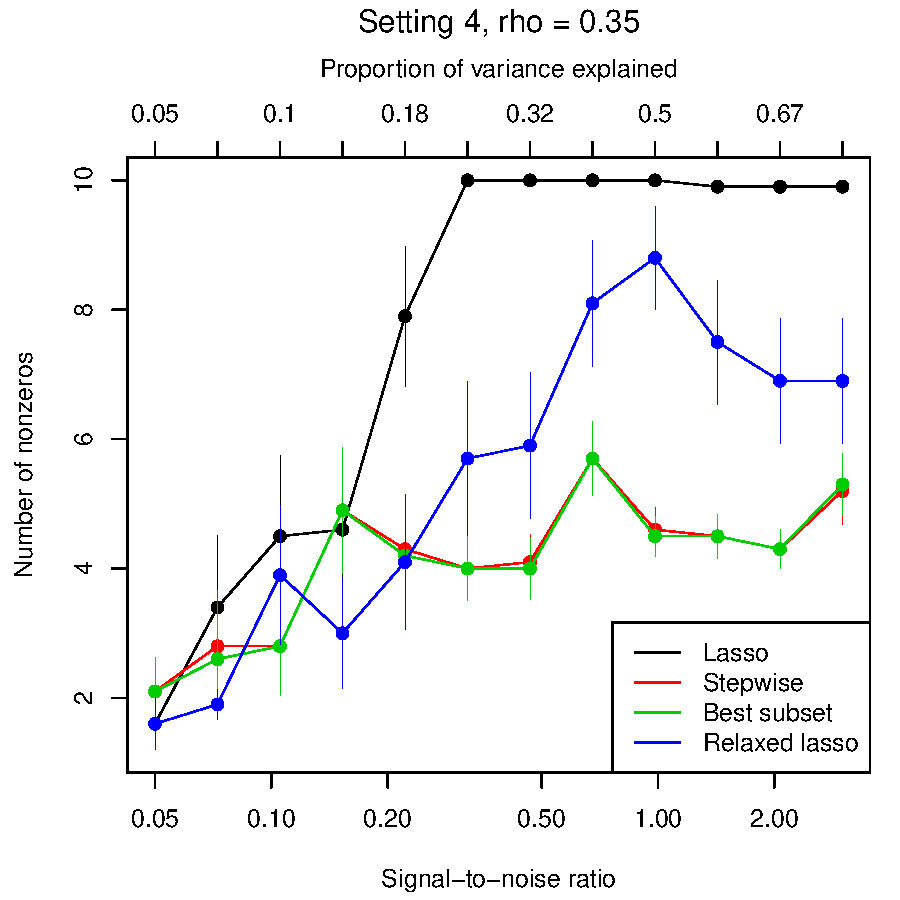
\includegraphics[width=0.32\textwidth]{{fig/val/nzs.sim.n100.p10.beta4.rho0.35}.pdf}
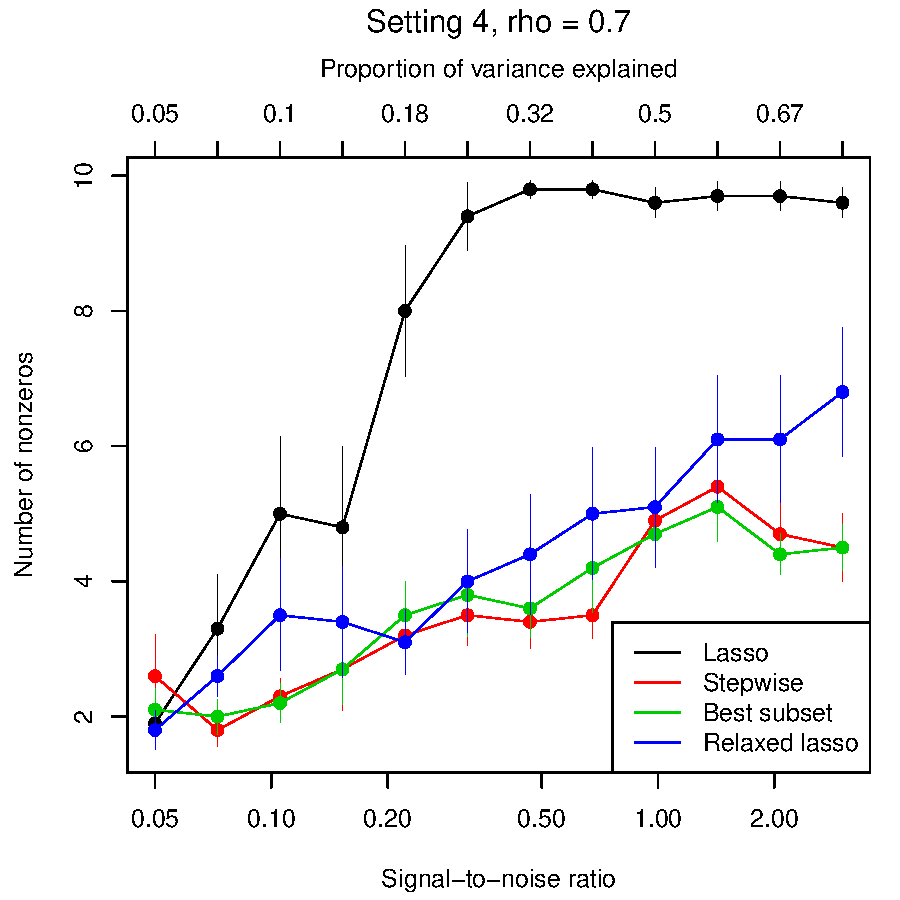
\includegraphics[width=0.32\textwidth]{{fig/val/nzs.sim.n100.p10.beta4.rho0.70}.pdf}
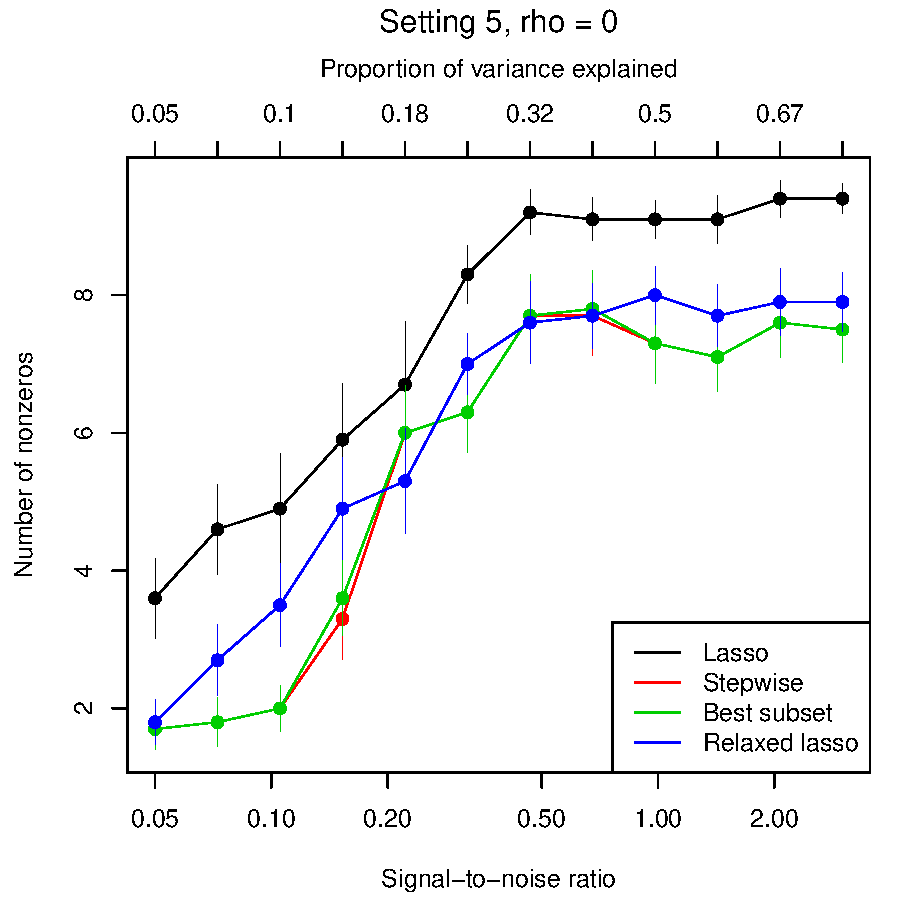
\includegraphics[width=0.32\textwidth]{{fig/val/nzs.sim.n100.p10.beta5.rho0.00}.pdf}
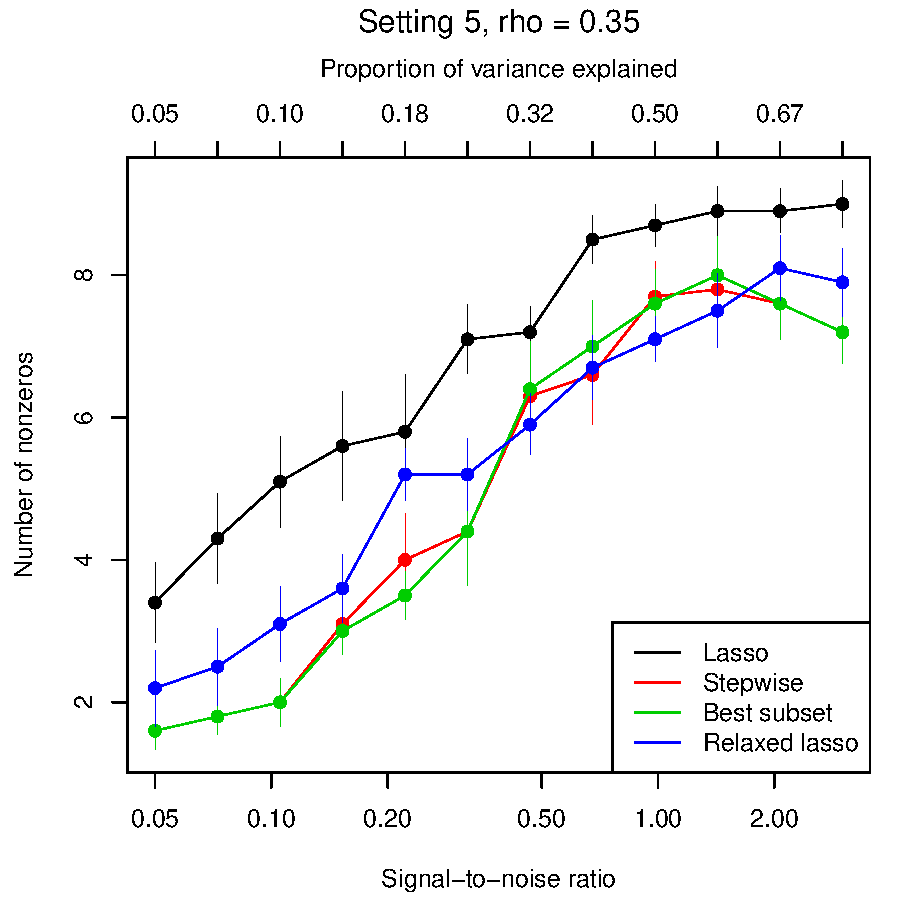
\includegraphics[width=0.32\textwidth]{{fig/val/nzs.sim.n100.p10.beta5.rho0.35}.pdf}
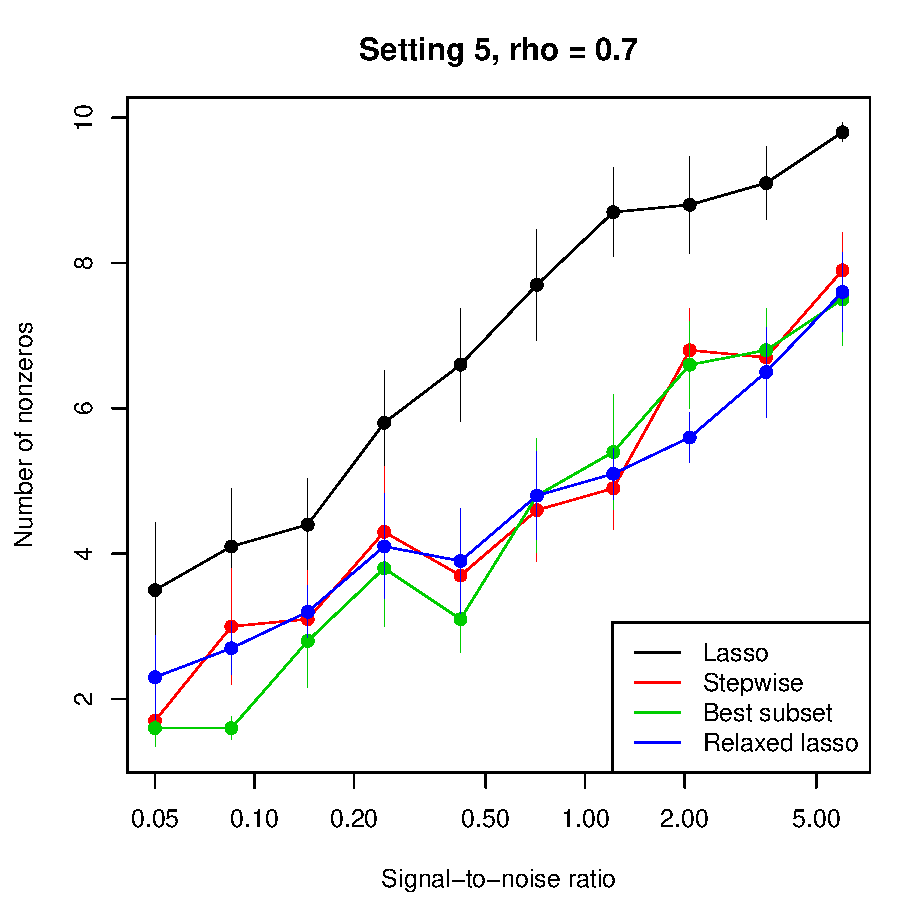
\includegraphics[width=0.32\textwidth]{{fig/val/nzs.sim.n100.p10.beta5.rho0.70}.pdf}

\end{figure}

\begin{figure}[p]
\centering
{\Large\bf $n=100$, $p=10$, Oracle tuning} \\
\bigskip
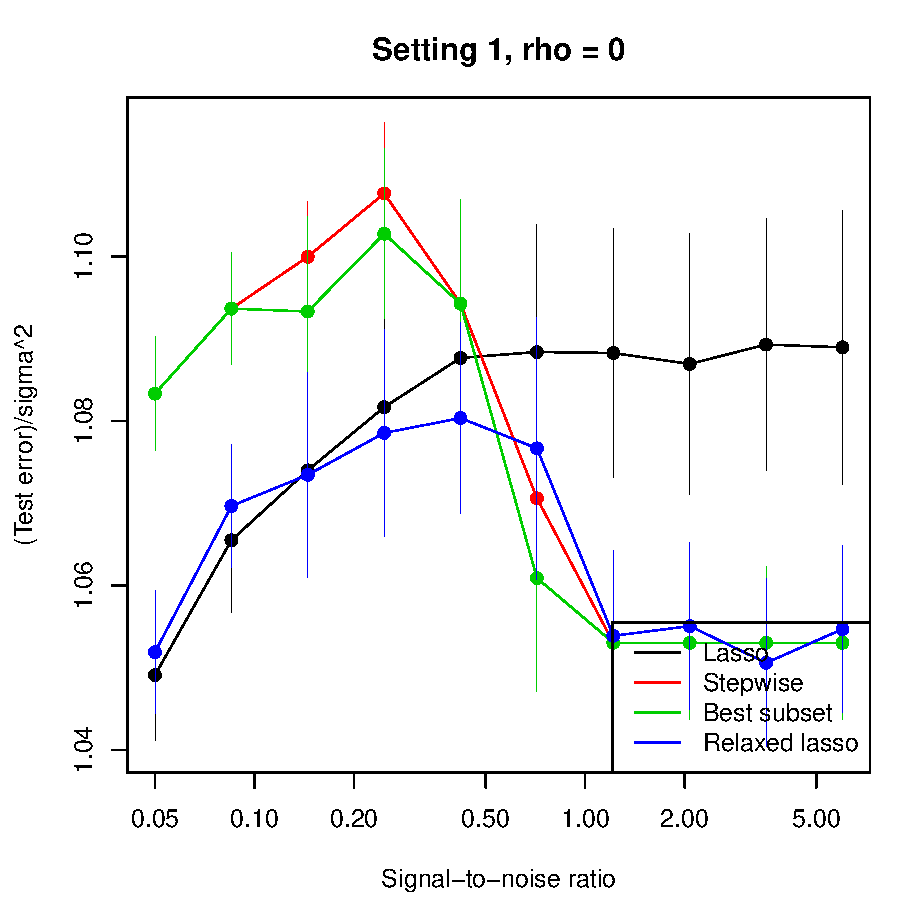
\includegraphics[width=0.32\textwidth]{{fig/val/err.sim.n100.p10.beta1.rho0.00}.pdf}
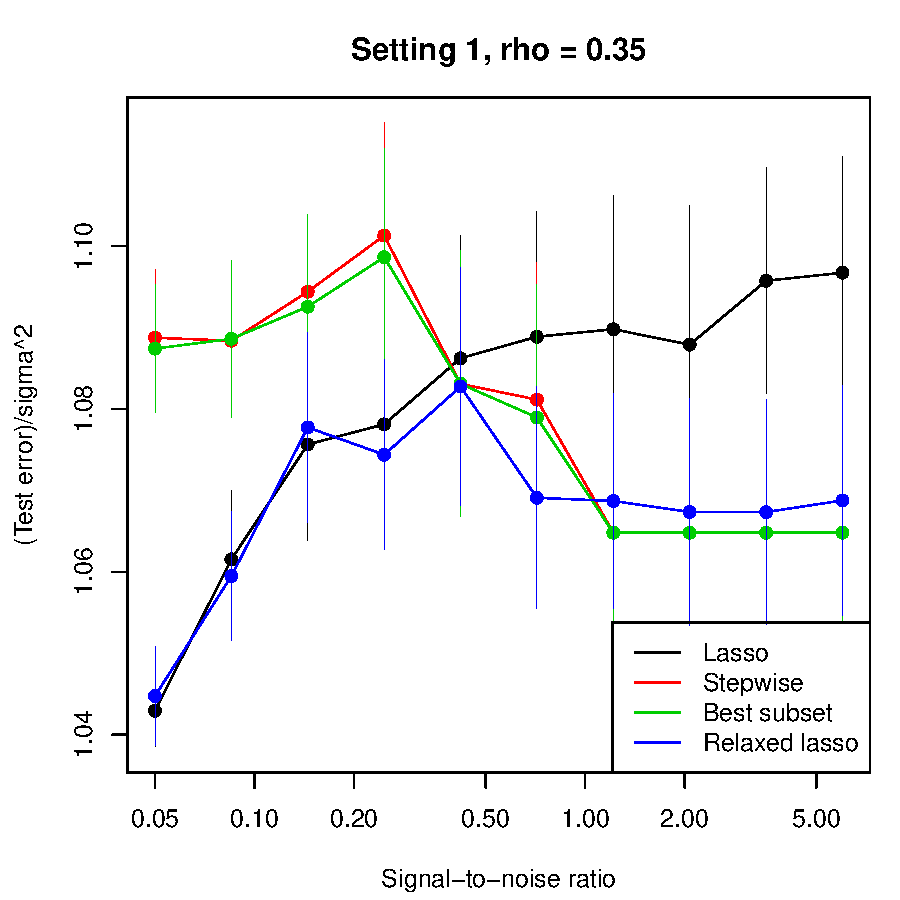
\includegraphics[width=0.32\textwidth]{{fig/val/err.sim.n100.p10.beta1.rho0.35}.pdf}
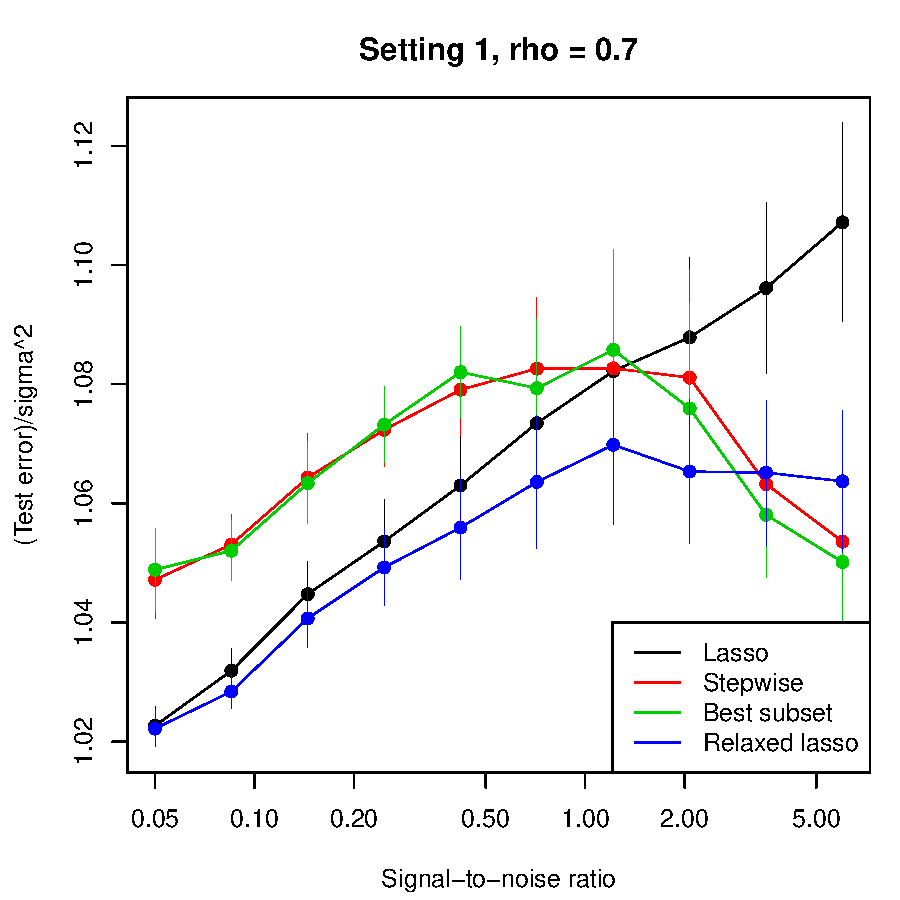
\includegraphics[width=0.32\textwidth]{{fig/val/err.sim.n100.p10.beta1.rho0.70}.pdf}
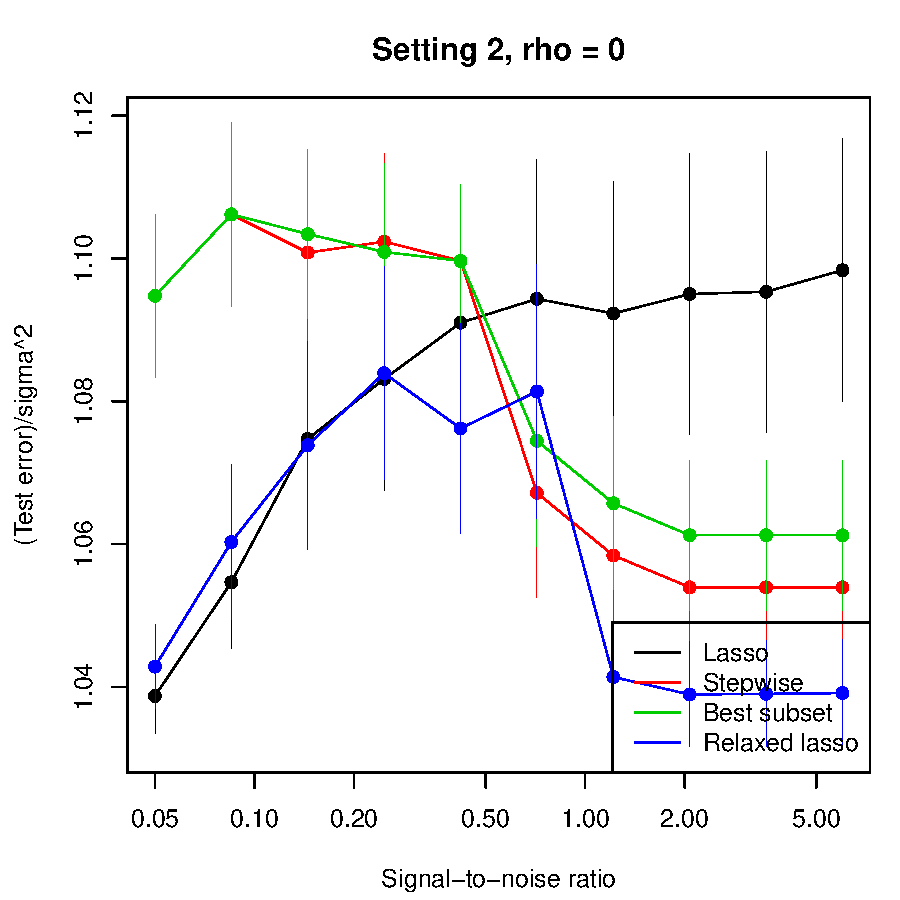
\includegraphics[width=0.32\textwidth]{{fig/val/err.sim.n100.p10.beta2.rho0.00}.pdf}
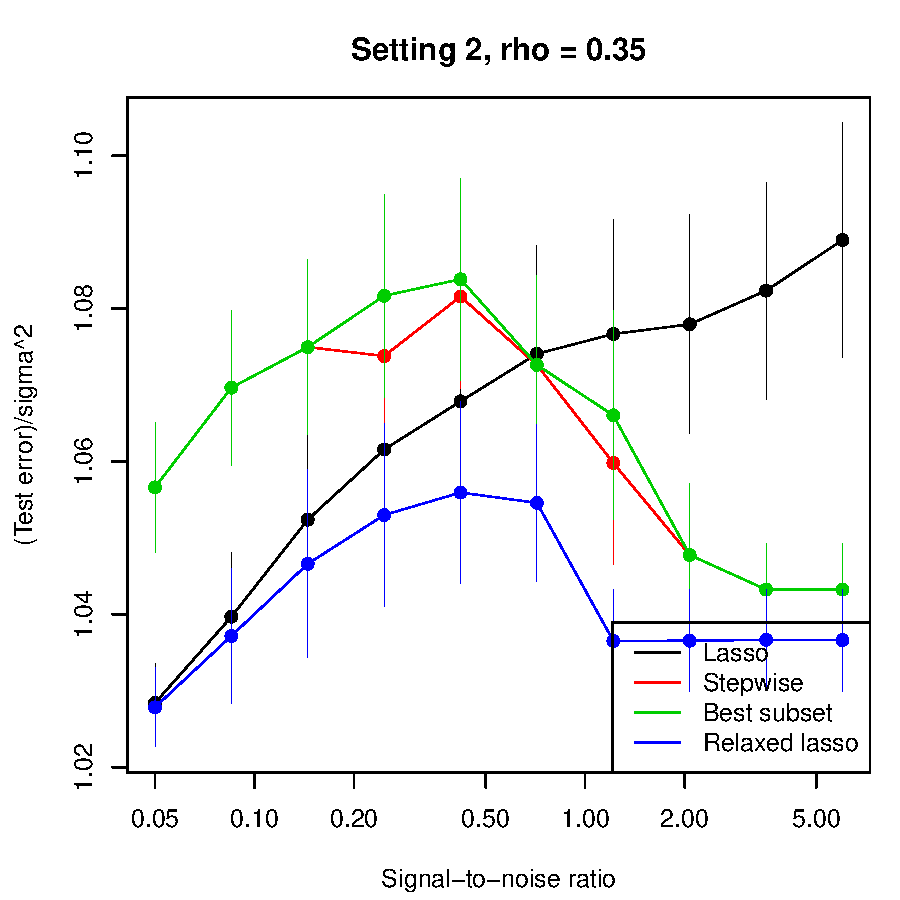
\includegraphics[width=0.32\textwidth]{{fig/val/err.sim.n100.p10.beta2.rho0.35}.pdf}
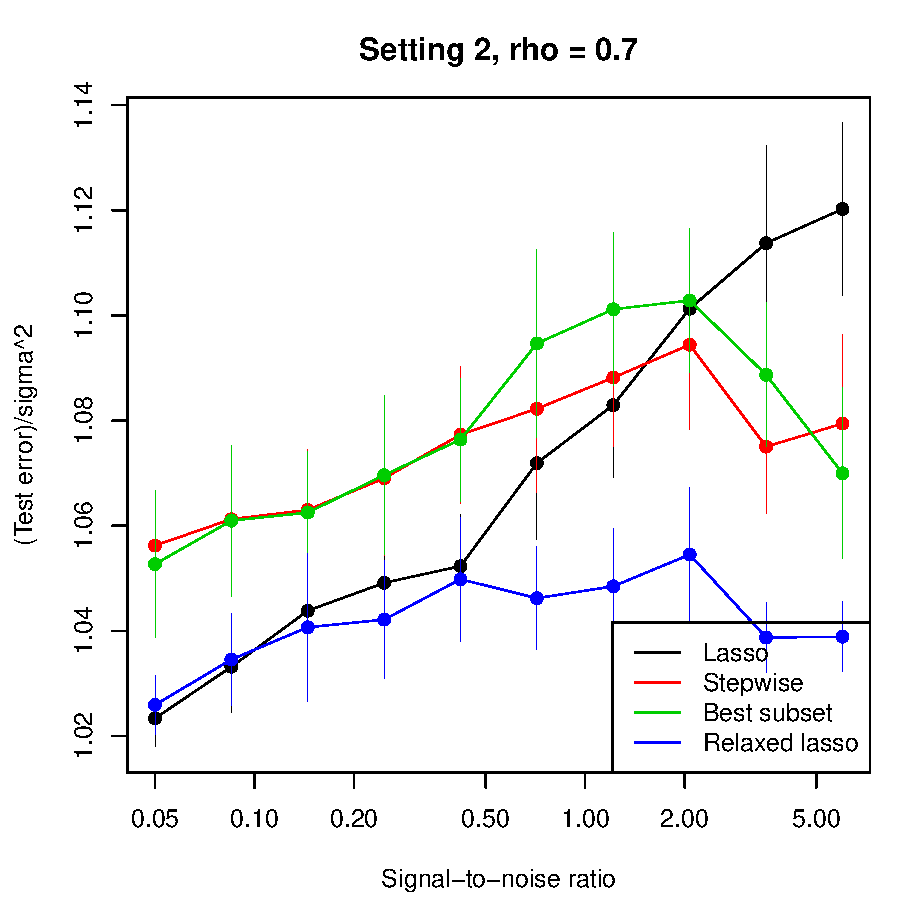
\includegraphics[width=0.32\textwidth]{{fig/val/err.sim.n100.p10.beta2.rho0.70}.pdf}
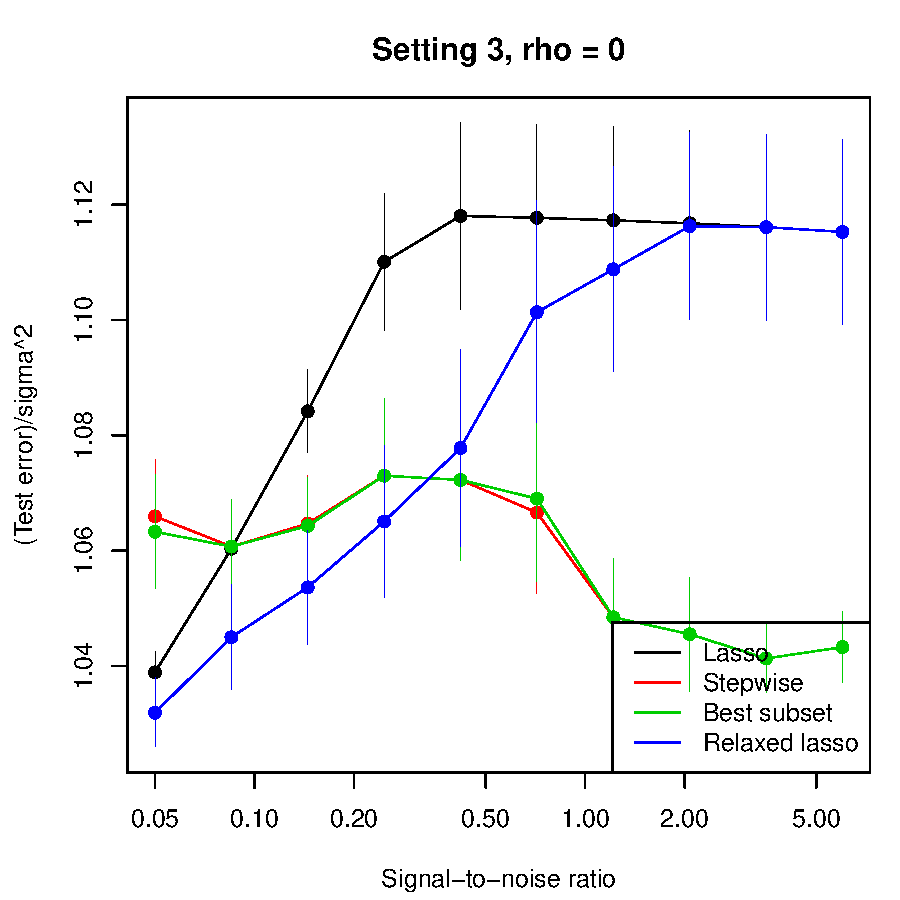
\includegraphics[width=0.32\textwidth]{{fig/val/err.sim.n100.p10.beta3.rho0.00}.pdf}
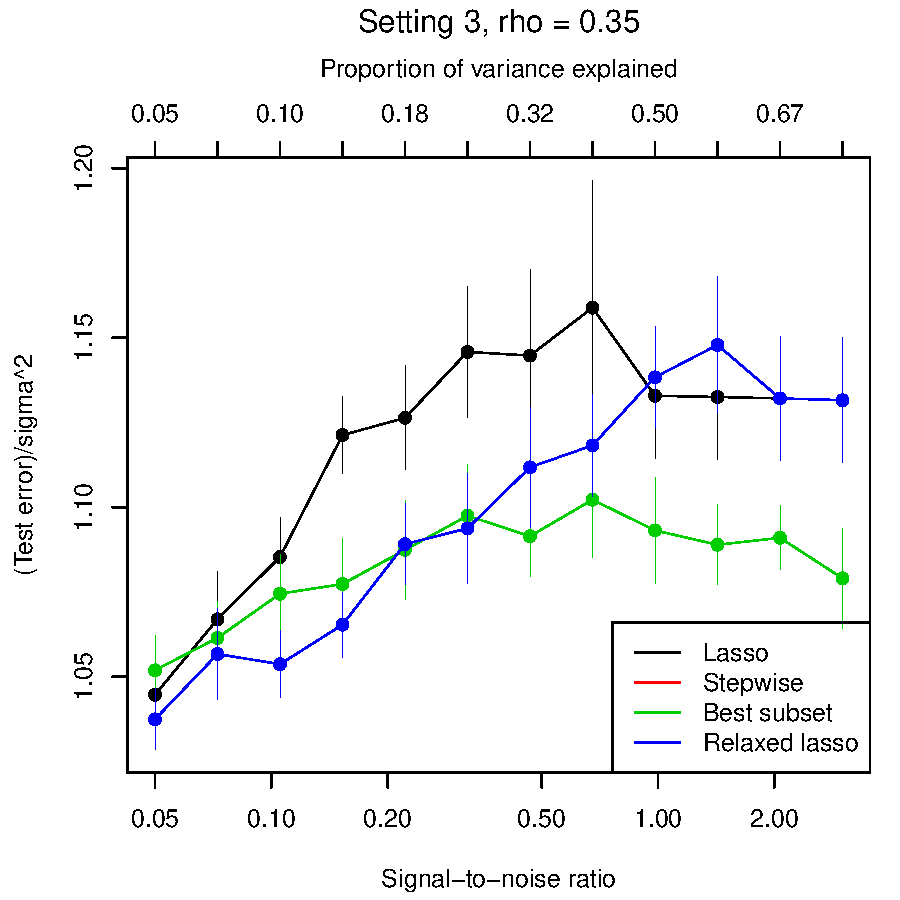
\includegraphics[width=0.32\textwidth]{{fig/val/err.sim.n100.p10.beta3.rho0.35}.pdf}
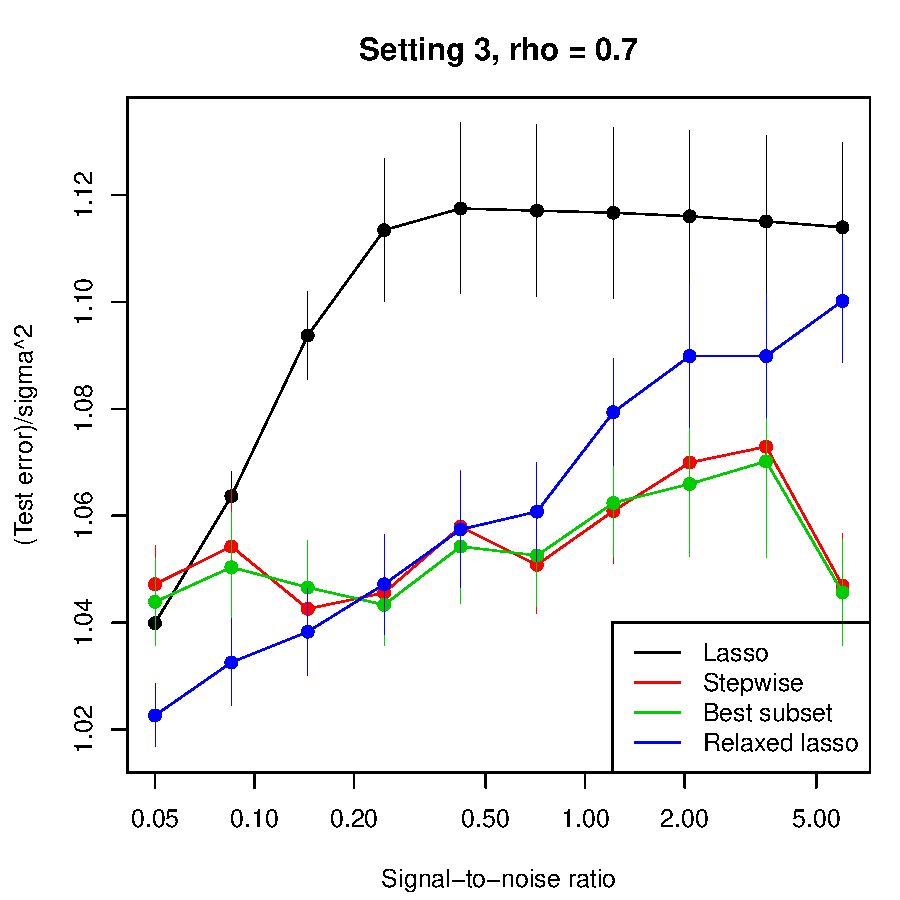
\includegraphics[width=0.32\textwidth]{{fig/val/err.sim.n100.p10.beta3.rho0.70}.pdf}
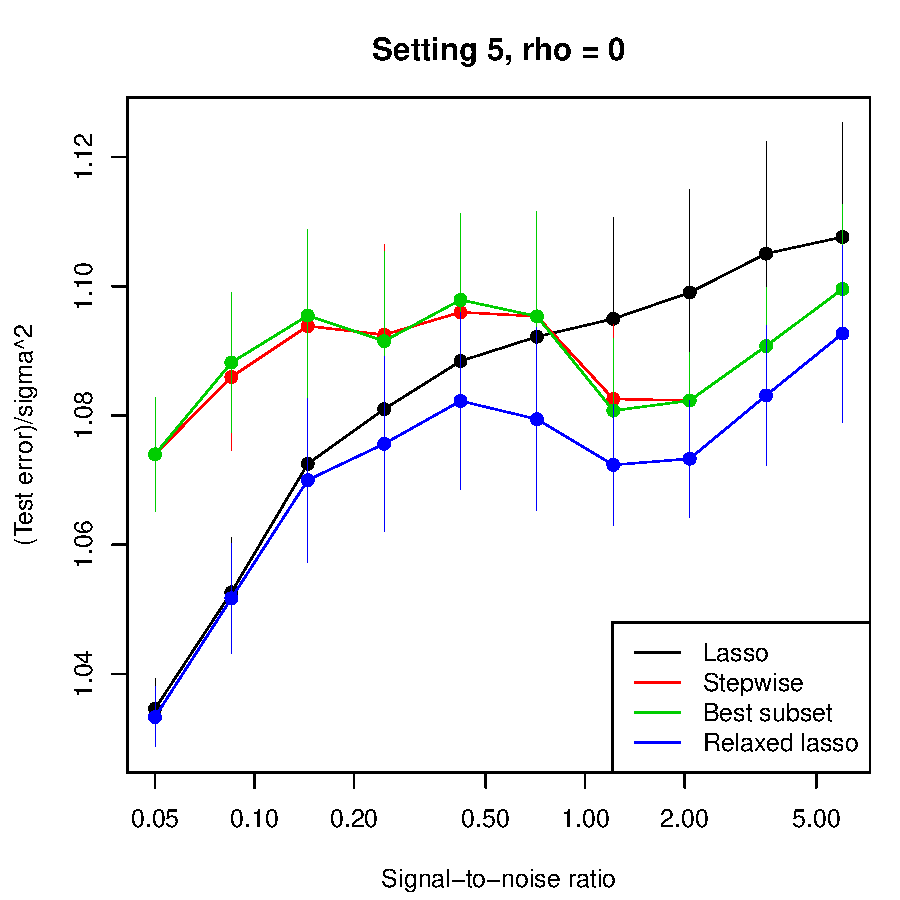
\includegraphics[width=0.32\textwidth]{{fig/val/err.sim.n100.p10.beta5.rho0.00}.pdf}
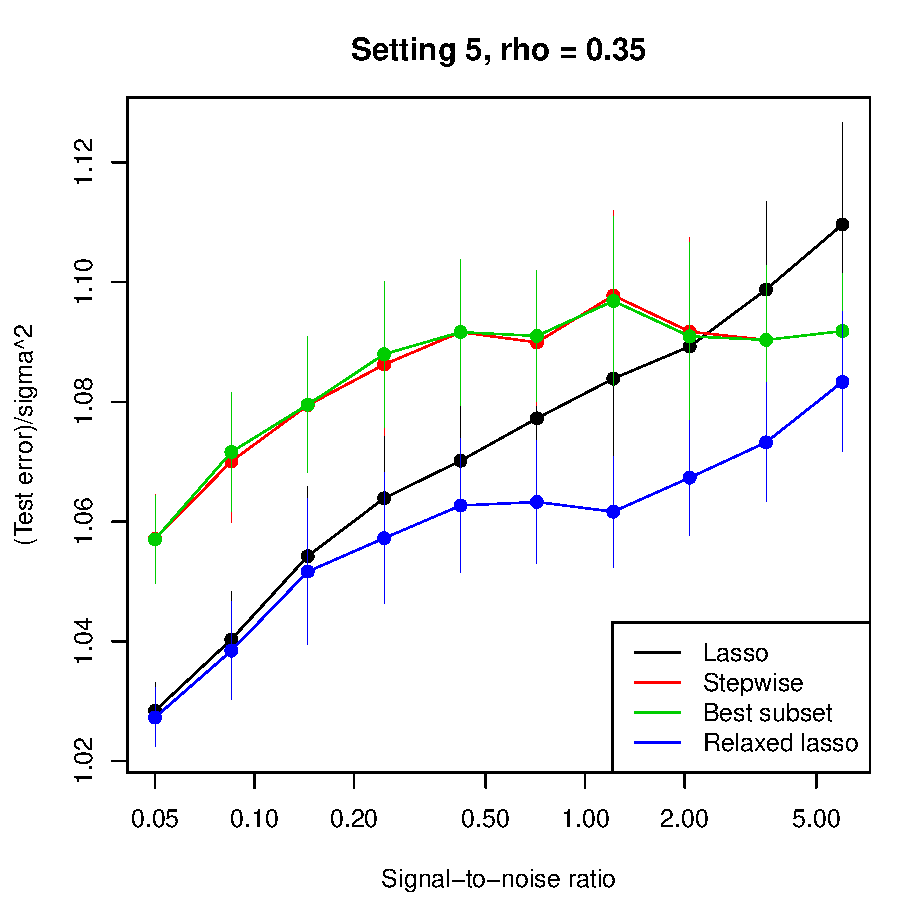
\includegraphics[width=0.32\textwidth]{{fig/val/err.sim.n100.p10.beta5.rho0.35}.pdf}
\includegraphics[width=0.32\textwidth]{{fig/val/err.sim.n100.p10.beta5.rho0.70}.pdf}

\end{figure}

\begin{figure}[p]
\centering
{\Large\bf $n=100$, $p=10$, Oracle tuning} \\
\bigskip
\includegraphics[width=0.32\textwidth]{{fig/val/pro.sim.n100.p10.beta1.rho0.00}.pdf}
\includegraphics[width=0.32\textwidth]{{fig/val/pro.sim.n100.p10.beta1.rho0.35}.pdf}
\includegraphics[width=0.32\textwidth]{{fig/val/pro.sim.n100.p10.beta1.rho0.70}.pdf}
\includegraphics[width=0.32\textwidth]{{fig/val/pro.sim.n100.p10.beta2.rho0.00}.pdf}
\includegraphics[width=0.32\textwidth]{{fig/val/pro.sim.n100.p10.beta2.rho0.35}.pdf}
\includegraphics[width=0.32\textwidth]{{fig/val/pro.sim.n100.p10.beta2.rho0.70}.pdf}
\includegraphics[width=0.32\textwidth]{{fig/val/pro.sim.n100.p10.beta3.rho0.00}.pdf}
\includegraphics[width=0.32\textwidth]{{fig/val/pro.sim.n100.p10.beta3.rho0.35}.pdf}
\includegraphics[width=0.32\textwidth]{{fig/val/pro.sim.n100.p10.beta3.rho0.70}.pdf}
\includegraphics[width=0.32\textwidth]{{fig/val/pro.sim.n100.p10.beta5.rho0.00}.pdf}
\includegraphics[width=0.32\textwidth]{{fig/val/pro.sim.n100.p10.beta5.rho0.35}.pdf}
\includegraphics[width=0.32\textwidth]{{fig/val/pro.sim.n100.p10.beta5.rho0.70}.pdf}

\end{figure}

\begin{figure}[p]
\centering
{\Large\bf $n=100$, $p=10$, Oracle tuning} \\
\bigskip
\includegraphics[width=0.32\textwidth]{{fig/val/nzs.sim.n100.p10.beta1.rho0.00}.pdf}
\includegraphics[width=0.32\textwidth]{{fig/val/nzs.sim.n100.p10.beta1.rho0.35}.pdf}
\includegraphics[width=0.32\textwidth]{{fig/val/nzs.sim.n100.p10.beta1.rho0.70}.pdf}
\includegraphics[width=0.32\textwidth]{{fig/val/nzs.sim.n100.p10.beta2.rho0.00}.pdf}
\includegraphics[width=0.32\textwidth]{{fig/val/nzs.sim.n100.p10.beta2.rho0.35}.pdf}
\includegraphics[width=0.32\textwidth]{{fig/val/nzs.sim.n100.p10.beta2.rho0.70}.pdf}
\includegraphics[width=0.32\textwidth]{{fig/val/nzs.sim.n100.p10.beta3.rho0.00}.pdf}
\includegraphics[width=0.32\textwidth]{{fig/val/nzs.sim.n100.p10.beta3.rho0.35}.pdf}
\includegraphics[width=0.32\textwidth]{{fig/val/nzs.sim.n100.p10.beta3.rho0.70}.pdf}
\includegraphics[width=0.32\textwidth]{{fig/val/nzs.sim.n100.p10.beta4.rho0.00}.pdf}
\includegraphics[width=0.32\textwidth]{{fig/val/nzs.sim.n100.p10.beta4.rho0.35}.pdf}
\includegraphics[width=0.32\textwidth]{{fig/val/nzs.sim.n100.p10.beta4.rho0.70}.pdf}
\includegraphics[width=0.32\textwidth]{{fig/val/nzs.sim.n100.p10.beta5.rho0.00}.pdf}
\includegraphics[width=0.32\textwidth]{{fig/val/nzs.sim.n100.p10.beta5.rho0.35}.pdf}
\includegraphics[width=0.32\textwidth]{{fig/val/nzs.sim.n100.p10.beta5.rho0.70}.pdf}

\end{figure}


\end{document}